% LTeX: enabled=false
% \iffalse meta-comment
% !TEX program  = pdfLaTeX
%<*internal>
\iffalse
%</internal>
%<*readme>
% LTeX: language=en-US
% LTeX: enabled=true
-----------------------------------------------------------------------------------------------------
fei --- Class for the creation of academic works under the typographic rules of FEI University Center
Author: Douglas De Rizzo Meneghetti
E-mail: douglasrizzo@fei.edu.br

Released under the LaTeX Project Public License v1.3c or later
See http://www.latex-project.org/lppl.txt
-----------------------------------------------------------------------------------------------------

fei is a class created by graduate students and LaTeX enthusiasts that allow students from FEI University Center to create their academic works, be it a monograph, master's thesis or PhD dissertation, under the typographic rules of the institution. The class makes it possible to create a full academic work, supporting functionalities such as cover, title page, catalog entry, dedication, summary, lists of figures, tables, algorithms, acronyms and symbols, multiple authors, index, references, appendices and attachments.

fei is loosely based in the Brazilian National Standards Organization (Associação Brasileira de Normas Técnicas, ABNT) standards for the creation of academic works, such as NBR 14724:2011, NBR 6023:2018 and NBR 10520:2002.
In the manual, users will find detailed information regarding the class commands, environments and best practices to create an academic text of good quality. We also made available a few template files which students may use as a starting point for their texts.

# License
Released under the LaTeX Project Public License v1.3c or later
See http://www.latex-project.org/lppl.txt

# Latest releases and version control
CTAN is always the place to go to get the stable version of the class. To know the changes done to the class and get previous and developments versions, visit https://www.github.com/douglasrizzo/Classe-Latex-FEI/.
% LTeX: enabled=false
%</readme>
%<*internal>
\fi
\def\nameofplainTeX{plain}
\ifx\fmtname\nameofplainTeX\else
  \expandafter\begingroup
\fi
%</internal>
%<*install>
\input docstrip.tex
\keepsilent
\askforoverwritefalse
\preamble
% LTeX: enabled=true
-----------------------------------------------------------------------------------------------------
fei --- Class for the creation of academic works under the typographic rules of FEI University Center
Author: Douglas De Rizzo Meneghetti
E-mail: douglasrizzo@fei.edu.br

Released under the LaTeX Project Public License v1.3c or later
See http://www.latex-project.org/lppl.txt
-----------------------------------------------------------------------------------------------------
\endpreamble
\postamble

Copyright (C) 2022 by Douglas De Rizzo Meneghetti <douglasrizzo@fei.edu.br>

This work may be distributed and/or modified under the
conditions of the LaTeX Project Public License (LPPL), either
version 1.3c of this license or (at your option) any later
version.  The latest version of this license is in the file:

http://www.latex-project.org/lppl.txt

This work is "maintained" (as per LPPL maintenance status) by
Douglas De Rizzo Meneghetti.

This work consists of the file  fei.dtx,
and the derived files           fei.pdf and
fei.cls.
% LTeX: enabled=false
\endpostamble
\usedir{tex/latex/fei}
\generate{
  \file{\jobname.cls}{\from{\jobname.dtx}{class}}
}
%</install>
%<install>\endbatchfile
%<*internal>
\usedir{source/latex/fei}
\generate{
  \file{\jobname.ins}{\from{\jobname.dtx}{install}}
}
\nopreamble\nopostamble
\usedir{doc/latex/fei}
\generate{
  \file{README.txt}{\from{\jobname.dtx}{readme}}
}
\ifx\fmtname\nameofplainTeX
  \expandafter\endbatchfile
\else
  \expandafter\endgroup
\fi
%</internal>
% \fi
% \iffalse
%<*driver>
\begin{filecontents*}{\jobname.xmpdata}
  \Title     {Classe LaTeX FEI}
  \Author    {Douglas De Rizzo Meneghetti}
  \Copyright {Copyright \copyright\ 2020 "Douglas De Rizzo Meneghetti"}
  \Keywords  {manual\sep latex\sep tipografia}
  \Publisher {Baking International}
  \Language  {pt-BR}
  \Subject   {This is where you put the abstract.}
\end{filecontents*}

\documentclass[nopdfa,oneside,symbols,acronym,font=times]{\jobname}
\usepackage{multicol}
\usepackage{listings}
\lstset{
basicstyle=\ttfamily,
columns=flexible,
breaklines=true,
literate=
  {ã}{{\~a}}1 {ẽ}{{\~e}}1 {ĩ}{{\~i}}1 {õ}{{\~o}}1 {ũ}{{\~u}}1
{Ã}{{\~A}}1 {Ẽ}{{\~E}}1 {Ĩ}{{\~I}}1 {Õ}{{\~O}}1 {Ũ}{{\~U}}1
{á}{{\'a}}1 {é}{{\'e}}1 {í}{{\'i}}1 {ó}{{\'o}}1 {ú}{{\'u}}1
{Á}{{\'A}}1 {É}{{\'E}}1 {Í}{{\'I}}1 {Ó}{{\'O}}1 {Ú}{{\'U}}1
{à}{{\`a}}1 {è}{{\`e}}1 {ì}{{\`i}}1 {ò}{{\`o}}1 {ù}{{\`u}}1
{À}{{\`A}}1 {È}{{\'E}}1 {Ì}{{\`I}}1 {Ò}{{\`O}}1 {Ù}{{\`U}}1
{ä}{{\"a}}1 {ë}{{\"e}}1 {ï}{{\"i}}1 {ö}{{\"o}}1 {ü}{{\"u}}1
{Ä}{{\"A}}1 {Ë}{{\"E}}1 {Ï}{{\"I}}1 {Ö}{{\"O}}1 {Ü}{{\"U}}1
{â}{{\^a}}1 {ê}{{\^e}}1 {î}{{\^i}}1 {ô}{{\^o}}1 {û}{{\^u}}1
{Â}{{\^A}}1 {Ê}{{\^E}}1 {Î}{{\^I}}1 {Ô}{{\^O}}1 {Û}{{\^U}}1
{œ}{{\oe}}1 {Œ}{{\OE}}1 {æ}{{\ae}}1 {Æ}{{\AE}}1 {ß}{{\ss}}1
{ű}{{\H{u}}}1 {Ű}{{\H{U}}}1 {ő}{{\H{o}}}1 {Ő}{{\H{O}}}1
{ç}{{\c c}}1 {Ç}{{\c C}}1 {ø}{{\o}}1 {å}{{\r a}}1 {Å}{{\r A}}1
{€}{{\euro}}1 {£}{{\pounds}}1 {«}{{\guillemotleft}}1
{»}{{\guillemotright}}1 {ñ}{{\~n}}1 {Ñ}{{\~N}}1
}
% LTeX: language=pt-BR
% LTeX: enabled=true
\author{Douglas De Rizzo Meneghetti}
\title{Classe \LaTeX{} da FEI para criação de trabalhos acadêmicos}
\subtitulo{de acordo com os guias de março de 2020 da biblioteca}
% \advisor{Donald Knuth}
% \curso{Formatação e Tipografia}

\newsubfloat{figure}

\newcommand{\bigvindex}[1]{\index{#1@\emph{#1}}\emph{#1}}
\newcommand{\vindex}[1]{\index{#1}#1}
\newcommand{\cfcite}[1]{(Cf. \textcite*{#1})}

\makeindex
\makeglossaries

\newacronym{fei}{FEI}{Fundação Educacional Inaciana}
\newacronym{abnt}{ABNT}{Associação Brasileira de Normas Técnicas}
\newacronym{abntex}{abn\TeX}{\emph{Absurd Norms for \TeX}}
\newacronym{cqd}{CQD}{como se queria demonstrar}
\newacronym[user1=\emph{quod erat demonstrandum}]{qed}{QED}{como se queria demonstrar}
\newacronym{ctan}{CTAN}{\emph{Comprehensive \TeX{} Archive Network}}

\newglossaryentry{h}{type=symbols, name={\ensuremath{H}}, sort=h, description={Esquema}}
\newglossaryentry{t}{type=symbols, name={\ensuremath{t}}, sort=t, description={Geração}}
\newglossaryentry{m}{type=symbols, name={\ensuremath{m}}, sort=m, description={número de cadeias pertences a \gls{h} na geração \gls{t}}}
\newglossaryentry{f}{type=symbols, name={\ensuremath{f}}, sort=f, description={aptidão média observada de \gls{h}}}
\newglossaryentry{at}{type=symbols, name={\ensuremath{a_t}}, sort=a, description={aptidão média observada na geração \gls{t}}}
\newglossaryentry{p}{type=symbols, name={\ensuremath{p}}, sort=p, description={probabilidade de ruptura de \gls{h}}}
\newglossaryentry{oh}{type=symbols, name={\ensuremath{o}}, sort=o, description={ordem de \gls{h}}}
\newglossaryentry{l}{type=symbols, name={\ensuremath{l}}, sort=l, description={tamanho do código}}
\newglossaryentry{pm}{type=symbols, name={\ensuremath{p_m}}, sort=pm, description={probabilidade de mutação}}
\newglossaryentry{pc}{type=symbols, name={\ensuremath{p_c}}, sort=pc, description={probabilidade de cruzamento}}
\newglossaryentry{delta}{type=symbols, name={\ensuremath{\delta}}, sort=delta, description={menor comprimento de \gls{h}}}

\addbibresource{referencias.bib}

\begin{document}

\maketitle

\begin{folhaderosto}
  Manual da classe \LaTeX{} da FEI apresentado como pré-requisito para que seus usuários saibam como utilizá-la.
\end{folhaderosto}
\fichacatalografica
\folhadeaprovacao
\dedicatoria{Esta dedicatória está aqui para que a função de dedicatória seja testada.}
\begin{agradecimentos}
  Agradecemos a Donald Knuth pela criação do \TeX{}, a Leslie Lamport pelo \LaTeX{} e a toda a comunidade de desenvolvedores que continua dando suporte e criando pacotes para melhorar a qualidade dos documentos escritos. Agradecimentos especiais são estendidos aos membros da \TeX{} \emph{Stack Exchange} pela divisão do fardo de criar documentos com belas tipografias. Agradece-se também os mantenedores da \gls{ctan}, por hospedar a classe e garantir sua distribuição em todas as maiores distribuições de \LaTeX{} nos principais sistemas operacionais, além de enviar-me e-mails toda vez que subo uma versão errada da classe.
\end{agradecimentos}

\begin{epigrafe}
  \epig{Beware of bugs in the above code; I have only proved it correct, not tried it.}{Donald E. Knuth \nocite{knuth77}}
  \epig{Something is rotten in the state of Denmark.}{William Shakespeare \nocite{shakespeare1885tragedy}}
\end{epigrafe}

% \epigrafe{A good scientist is a person with original ideas. A good engineer is a person who makes a design that works with as few original ideas as possible. There are no prima donnas in engineering.}{Freeman Dyson \nocite{dyson_disturbing_1979}}

\begin{resumo}
  O \TeX{} é um sistema de formatação de textos baseado em uma \emph{mark-up language}, criado em 1978 por Donald Knuth e ampliado com uma série de macros por Leslie Lamport, dando à luz o \LaTeX{}. Usado com frequência na área acadêmica, foram criadas classes em \LaTeX{} para satisfazer às regras de formatação dos mais variados órgãos, sociedades, institutos e universidades. Baseada nos padrões da ABNT, a biblioteca da FEI criou seu próprio guia para formatação de trabalhos acadêmicos, o qual originou, extra-oficialmente, a classe \LaTeX{} da FEI. Neste guia, os usuários serão guiados no uso dessa classe, desde a criação de elementos pré-textuais (capa, folha de rosto, ficha catalográfica, epígrafe, dedicatória, sumário, listas de figuras, tabelas, algoritmos, siglas e símbolos), passando pelo corpo do texto e elementos pós-textuais (índice remissivo, referências bibliográficas, apêndices e anexos) e terminando com uma explicação referente à instalação dos pré-requisitos e compilação de um trabalho dissertativo com todos os recursos que a classe pode oferecer.
  \keywords{\LaTeX{}. FEI.}
\end{resumo}

\begin{abstract}
  Abstract goes here.
  \keywords{Keywords. Go. Here.}
\end{abstract}

\listoffigures
\listoftables
\listofalgorithms
\listoftheorems
\printglossaries
\tableofcontents

\chapter{Introdução}

\glsaddall%
A biblioteca do Centro Universitário \index{FEI}\gls{fei} disponibiliza um guia de formatação de monografias de graduação, mestrado e doutorado. Usando tanto o guia, como algumas dúzias de trabalhos corrigidos pelas bibliotecárias e e-mails e visitas incessantes da minha parte à biblioteca, nasceu a classe \LaTeX{} da \gls{fei}, especializada na criação de trabalhos acadêmicos sob as normas da biblioteca da \gls{fei}. Com ela, os alunos podem usar seus conhecimentos em \LaTeX{} para criar seus documentos, deixando a maior parte da formatação complexa do documento a cargo da classe. Espera-se que os autores tenham menos trabalho com a formatação do texto do que com a escrita do mesmo.

A classe redefine alguns comandos e ambientes pré-existentes do \LaTeX{} e cria novos comandos e ambientes. Todos eles são descritos neste manual.

Este manual é organizado da seguinte forma: a seção \ref{chap:introducao} lista os passos para instalação do \LaTeX{}, da classe e de suas dependências nos principais sistemas operacionais; a seção \ref{chap:comandos} enumera os comandos e ambientes, tanto novos quanto redefinidos do \LaTeX{}, necessários para a criação do corpo do trabalho acadêmico; a seção \ref{chap:referencia} explica o uso do abn\TeX{} e exemplifica o uso de seus diversos comandos de citação; a seção \ref{chap:indice} disserta sobre os programas necessários para a criação do índice remissivo e os comandos usados para se indexar termos no decorrer do texto; a seção \ref{chap:listas} explica ao autor como criar listas de abreviaturas e símbolos; a seção \ref{chap:compilando} ensina a compilar um projeto usando a classe \LaTeX{} da FEI com todas as suas funcionalidades. O apêndice~\ref{app:hacks} descreve alguns \emph{hacks} úteis para usuários da classe que precisam realizar as customizações mais corriqueiras na formatação de seus trabalhos Já o apêndice~\ref{app:arquivos} explica cada um dos arquivos criados pelo processo de compilação, com o propósito de instruir e exemplificar o uso de um apêndice. Por último, o apêndice~\ref{app:simbolos} disponibiliza uma lista dos principais símbolos matemáticos disponíveis no \TeX{}.

\section{Dúvidas, problemas e contribuições}%
\label{chap:faq}

Este manual descreve como produzir um documento usando a classe da FEI. Caso tenha dúvidas relacionadas a editores de texto, serviços online (como o Overleaf\index{Overleaf}), problemas frequentes de compilação ou geração de referências, existe uma wiki\index{wiki} no GitHub\index{GitHub}: \url{https://github.com/douglasrizzo/Classe-Latex-FEI/wiki}

Os \emph{issues} do GitHub\index{GitHub} listam os problemas já conhecidos que a classe tem. Lá é o local preferencial para reportar problemas relacionados a ela: \url{https://github.com/douglasrizzo/Classe-Latex-FEI/issues}

\section{Instalação}%
\label{chap:instalacao}

A instalação do \LaTeX{} e da classe foram movidas para a Wiki, cujo endereço está disponível na seção~\ref{chap:faq}.

\section{Fonte Arial}

Por ser uma fonte True Type de autoria da Microsoft, as fontes da família Arial\index{Arial} não são disponibilizadas nativamente por distribuições do \LaTeX{} como o Mik\TeX{} e o \TeX{} \emph{Live}. Para utilizá-las, é necessário instalá-las separadamente. As instruções para instalação das fontes estão disponíveis no site do \TeX \emph{Users Group}\footnote{http://tug.org/fonts/getnonfreefonts/}.

\begin{itemize}
  \item Fazer download do script\footnote{http://tug.org/fonts/getnonfreefonts/install-getnonfreefonts};
  \item Instalar o script usando o aplicativo \texttt{texlua}: \lstinline+texlua install-getnonfreefonts+;
  \item Rodar o script: \lstinline+getnonfreefonts --all+.
\end{itemize}

Após isso, é possível usar a opção \texttt{font=arial} na declaração da classe, no início do arquivo \texttt{tex}: \lstinline+\documentclass[font=arial]{fei}+.

Alternativamente, é possível usar a fonte Arimo\index{Arimo}, uma versão aberta da fonte Arial disponibilizada nas principais distribuições de \LaTeX{}. Para isso, basta ter o pacote \texttt{arimo} instalado e usar a opção \texttt{font=arimo} na declaração da classe.

\section{Dependências}%
\label{sec:dependencias}

A partir da versão 3, a classe da FEI foi criada tendo a classe \texttt{memoir} como base, o que permitiu com que a classe fosse personalizada, em sua maioria, através do uso de comandos nativos do \LaTeX{}, reduzindo o número de pacotes do qual ela depende.

No entanto, ainda é necessário enfatizar a necessidade de instalação de alguns pacotes, listados abaixo, dos quais a classe \LaTeX{} da FEI depende para seu funcionamento correto. Estes pacotes estão disponíveis nas distribuições do Mik\TeX{} (para Windows), Mac\TeX{} (para Mac OS) e \TeX{} \emph{Live} (para Linux e Mac OS):\footnote{Como uma ironia do destino, o guia da biblioteca permite alíneas alfabéticas e a lista de pacotes possui mais de 26 itens, o que impede que ela seja representada como uma alínea.}
\texttt{algorithm2e},
\texttt{amsthm},
\texttt{arimo},
\texttt{babel},
\texttt{biblatex},
\texttt{biblatex-abnt},
\texttt{chngcntr},
\texttt{csquotes},
\texttt{enumitem},
\texttt{fontenc},
\texttt{glossaries},
\texttt{glossaries-extra},
\texttt{graphicx},
\texttt{hyperref},
\texttt{icomma},
\texttt{ifthen},
\texttt{imakeidx},
\texttt{inputenc},
\texttt{kvoptions},
\texttt{lmodern},
\texttt{mathtools},
\texttt{mfirstuc},
\texttt{microtype},
\texttt{morewrites},
\texttt{newtx},
\texttt{pdfpages},
\texttt{pdfx},
\texttt{thmtools},
\texttt{urwchancal} e
\texttt{xfor}.

Os scripts de alguns programas \TeX{}, como o \texttt{makeglossaries}, são dependentes da linguagem \index{Perl}Perl, a qual vem instalada por padrão em alguns sistemas operacionais. Para os usuários de Windows, no entanto, o Perl deve ser instalado separadamente e pode ser encontrado em \url{https://www.perl.org/}.

\chapter{Comandos e ambientes}%
\label{chap:comandos}

Esta seção descreve os comandos disponibilizados pela classe. Ele é separado em quatro seções: a seção \ref{sec:preambulo} disserta sobre os comandos a serem usados antes do início do texto; a seção \ref{sec:pretexto} auxilia na declaração dos elementos pré-textuais do documento; a seção \ref{sec:texto} descreve a estrutura do texto e outros elementos a serem usados durante a produção deste, como \emph{floats}; a seção \ref{sec:postexto} disserta sobre os elementos pós-textuais, a saber, referências, apêndices, anexos e índice remissivo.

\section{Preâmbulo}%
\label{sec:preambulo}

No preâmbulo do texto são declaradas as propriedades globais do documento, como a classe que rege a formatação geral do texto e novos comandos a serem usados no decorrer do texto. O preâmbulo da classe \LaTeX{} da FEI contém os seguintes elementos que devem ser declarados no preâmbulo:

\subsection{Metadados PDF/A}%
\label{subsec:pdfa}

A partir de 2017, os trabalhos depositados na biblioteca da instituição devem aderir ao padrão PDF/A, um formato voltado ao arquivamento de documentos PDF e disponibilização dos metadados e texto do documento para buscas.

A classe da FEI implementa a forma mais bem suportada de aderência ao padrão PDF/A disponível na comunidade \TeX{}, através do pacote \texttt{xpdf}. Contudo, a aderência total ao padrão é praticamente impossível sem minar as liberdades dos usuários com relação a como criam seus textos.

Por exemplo, o padrão PDF/A é quebrado caso um usuário insira figuras em formato vetorial, como EPS e PDF, caso essas figuras não estejam em conformidade com o padrão PDF/A. O padrão também e quebrado caso novas fontes ou símbolos sejam usados no documento, casos esses não possam ser convertidos para Unicode.

Dito isso, a forma correta de \emph{tentar} a aderência ao padrão é a que se segue.

Para que o arquivo PDF seja gerado com os metadados relevantes, um arquivo com o nome do arquivo \texttt{.tex} principal, porém com extensão \texttt{.xmpdata}, deve existir no diretório-raiz do projeto contendo tais metadados. Os usuários da classe da FEI não precisam criar este documento manualmente, podendo apenas inserir as seguintes linhas antes do comando \lstinline+\documentclass+, modificando os metadados de interesse.

\begin{lstlisting}
\begin{filecontents*}{\jobname.xmpdata}
\Title     {Minha tese-dissertação-monografia}
\Author    {Meu Nome\sep Nome Do Outro Integrante\sep Nome do Terceiro}
\Copyright {Copyright \copyright\ 2022 "Douglas De Rizzo Meneghetti"}
\Keywords  {manual\sep latex\sep tipografia}
\Language  {pt-BR}
\Subject   {Resumo vai aqui em uma única linha corrida.}
\end{filecontents*}
\end{lstlisting}

Uma lista com mais opções de metadados está disponível em \url{https://www.mathstat.dal.ca/~selinger/pdfa/sample.xmpdata}.

Para se validar a aderência ao formato PDF/A, recomenda-se o uso do \emph{veraPDF}\footnote{\url{https://verapdf.org/software/}}, um software padrão, gratuito e multiplafatorma. Também é possível usar o Adobe Acrobat Pro.

\subsection{Declaração da classe}%
\label{subsec:documentclass}

A declaração da classe é feita da seguinte forma:

\begin{lstlisting}
\documentclass[opções]{fei}
\end{lstlisting}

A classe da FEI pode receber as seguintes opções:

\begin{enumerate}
  \item \texttt{draft}: Essa opção simplifica o processo de compilação do PDF para que ele seja realizado mais rapidamente. A opção beneficia especialmente a compilação de trabalhos com um número elevado de imagens ou que incluam imagens cujos arquivos sejam grandes, uma vez que as imagens não são adicionadas ao PDF. \emph{Hyperlinks} internos (\emph{e.g. links} para seções, citações, símbolos, abreviaturas, figuras, tabelas) também não são inseridos\footnote{Para uma lista mais completa das mudanças advindas do uso da opção \texttt{draft}, cheque o seguinte tópico no StackExchange: \url{https://tex.stackexchange.com/q/49277/30998}.};
  \item \texttt{nopdfa}: desabilita a geração do documento no formato PDF/A. Essa função é disponibilizada para fins de compatibilidade, para que trabalhos antigos que possivelmente sejam corrompidos durante o processo de compilação devido ao padrão PDF/A ainda possam ser compilados;
  \item \texttt{deposito}: Procura por arquivos PDF referentes à ficha catalográfica\index{ficha catalográfica} e folha de aprovação\index{folha de aprovação} no diretório do documento e os insere nos locais em que \lstinline+\fichacatalografica+ e \lstinline+\folhadeaprovacao+ são chamados. Caso contrário, insere páginas indicativas, para fins de contagem de número de páginas;
  \item \texttt{sublist}: configura o pacote \texttt{glossaries} para que sub-listas de símbolos sejam usadas. Mais sobre sub-listas na seção \ref{sec:sublist};
  \item \texttt{numeric}: troca as citações e referências autor-data para numéricas;
  \item \texttt{algo-as-figure}: configura o pacote \texttt{algorithm2e} para que algoritmos sejam listados na lista de ilustrações. Essa configuração é preferível, uma vez que a formatação das legendas e da lista de algoritmos, no presente, não condiz com as recomendações do guia da biblioteca;
  \item \texttt{twoside}: a atualização de 2015 do guia da biblioteca recomenda que trabalhos acadêmicos com mais de 100 páginas sejam impressos em formato \index{frente-e-verso}frente-e-verso. Por ser derivada da classe \texttt{memoir}, a classe da FEI pode receber algumas opções nativas de \texttt{memoir}. Um exemplo de opção que pode ser útil é \texttt{twoside}, a qual alterna o tamanho das margens direita e esquerda das páginas, assim como a posição da numeração, gerando um documento frente-e-verso da forma correta. Alterações adicionais foram realizadas para que todos os elementos pré-textuais sejam corretamente iniciados nas páginas ímpares, como recomenda o guia e a norma. É importante reparar, contudo, que a utilização de \texttt{twoside} acarreta no aumento do número de páginas, uma vez que os versos de algumas páginas no pré-texto podem ser deixados em branco em prol da norma.
  \item \texttt{acronym}: passado para o pacote \texttt{glossaries-extra}, sinaliza o uso de abreviaturas no trabalho;
  \item \texttt{symbols}: passado para o pacote \texttt{glossaries-extra}, sinaliza o uso de símbolos no trabalho;
  \item \texttt{backrefs}: passa a opção \texttt{backref} ao pacote \texttt{biblatex}, para que ele imprima as páginas nas quais cada trabalho foi citado nas referências bibliográficas. Esta não é uma funcionalidade prevista no guia de formatação de referências da biblioteca, mas pode ser útil no caso de bancas que gostam de checar se o aluno citou de fato todos os documentos listados nas referências. Apenas lembre-se de tirar isso antes da entrega final;
  \item \texttt{record}: passado para o pacote \texttt{glossaries-extra}, sinaliza o uso de um arquivo \texttt{.bib} para definição de símbolos e abreviaturas, a ser compilado pelo programa \index{bib2gls@\texttt{bib2gls}}\texttt{bib2gls};
  \item \texttt{abbr-shortcuts}: ativa a opção \texttt{shortcuts=abbr} para o pacote \texttt{glossaries-extra}. Ver seção~\ref{sec:citar-abrevs-simbs} e seção 4.3 do manual do \texttt{glossaries-extra} para mais informações.
\end{enumerate}

\subsection{Nome do autor, e título}

O nome do autor e o título da obra são inseridos usando os comandos nativos do \LaTeX{} \lstinline+\author{author}+ e \lstinline+\title{title}+. Eles são posteriormente usados na criação da capa e folha de rosto do trabalho, formatados sob as normas da biblioteca. Para trabalhos com mais de um autor, os nomes dos autores devem ser separados pelo comando \lstinline+\and+ ou \lstinline+\\+, como no exemplo:

\begin{lstlisting}
\author{Leonardo Anjoletto Ferreira \and Douglas De Rizzo Meneghetti}
\end{lstlisting}

\subsection{Subtítulo (opcional)}

Uma vez que as normas da biblioteca demandam formatações específicas para o título e subtítulo do documento (título em letras maiúsculas na capa, seguido do subtítulo em letras normais, separados por ``:''), foi criado o comando \lstinline+\subtitulo{}+, o qual recebe o texto referente ao subtítulo do texto. Este comando pode ser usado, preferencialmente, após o comando \lstinline+\title{}+ no preâmbulo do documento. Título e subtítulo também aparecem na folha de rosto.

\subsection{Cidade e Instituição (opcionais)}
Os comandos \lstinline+\cidade{}+ e \lstinline+\instituicao{}+ recebem os nomes da cidade e instituição de ensino para substituí-los na capa e folha de rosto. São comandos opcionais criados por questão de compatibilidade, ou caso outras instituições queiram usar a classe. Seus valores-padrão são ``São Bernardo do Campo'' e ``Centro Universitário FEI'', respectivamente.

\subsection{Arquivos de referências bibliográficas}%
\label{subsec:referencias-pre}

Em \TeX{}, as referências bibliográficas são mantidas em um ou mais arquivos de extensão \texttt{bib}, preferencialmente no mesmo diretório do arquivo \texttt{tex} do trabalho. Os arquivos \texttt{bib} usados pelo trabalho devem ser referenciados no preâmbulo do texto usando o comando \lstinline+\addbibresource{ref.bib}+. Mais de um arquivo pode ser referenciado, usando-se o comando \lstinline+\addbibresource{}+ mais de uma vez.

Para saber como imprimir a lista de referências bibliográficas na seção pós-textual so trabalho, confira a seção \ref{subsec:referencias-pos}.

\section{Pré-texto}%
\label{sec:pretexto}

O pré-texto do documento engloba todos os elementos textuais que precedem o corpo da obra. A seguir são listados os elementos pré-textuais suportados pela classe \LaTeX{} da FEI e os respectivos comandos para a criação de cada um deles.

\subsection{Capa}

A capa do trabalho é inserida através do comando \lstinline+\maketitle+, o qual foi modificado para criar uma página no formato da biblioteca. O comando usa o nome fornecido em \lstinline+\author{}+, o título em \lstinline+\title{}+, o subtítulo de \lstinline+\subtitulo{}+ juntamente com o ano corrente para gerar a capa.

\subsection{Folha de rosto}

A folha de rosto recebe um texto pré-definido, de acordo com o nível do trabalho escrito (monografia, dissertação ou tese). Este texto pode ser encontrado no guia da biblioteca e deve ser colocado dentro do ambiente \texttt{folhaderosto}. Por exemplo,
\begin{lstlisting}
\begin{folhaderosto}
Dissertação de Mestrado apresentada ao Centro Universitário
da FEI para obtenção do título de Mestre em Engenharia
Elétrica, orientado pelo Prof. Dr. Nome do Orientador.
\end{folhaderosto}
\end{lstlisting}

\subsection{Ficha catalográfica e folha de aprovação}

Os comandos \lstinline+\fichacatalografica+ e \lstinline+\folhadeaprovacao+ inserem páginas indicativas dos locais onde a ficha catalográfica e a folha de aprovação serão inseridas no trabalho. Caso a opção \lstinline+deposito+ seja passada à classe, o comando \lstinline+\folhadeaprovacao+ procura pelo arquivo \texttt{ata.pdf} na pasta raiz do arquivo \texttt{tex} e o insere no documento. O comando \lstinline+\fichacatalografica+ executa uma função semelhante, procurando pelo arquivo \texttt{ficha.pdf}.

\subsection{Dedicatória}

O comando \lstinline+\dedicatoria{}+ recebe um argumento com a dedicatória desejada e o insere na posição especificada pelo guia da biblioteca. Por exemplo: \\ \lstinline+\dedicatoria{A quem eu quero dedicar o texto}+.

\subsection{Agradecimentos}

O ambiente de agradecimentos não possui nenhuma propriedade especial, somente centraliza o título e deixa o texto que se encontra entre seu \texttt{begin} e \texttt{end} na formatação esperada.

\begin{lstlisting}
\begin{agradecimentos}
A quem se deseja agradecer.
\end{agradecimentos}
\end{lstlisting}

\subsection{Epígrafe}

A página da epígrafe é criada usando o ambiente \texttt{epigrafe}. Dentro deste ambiente, uma ou mais citações podem ser inseridas separadamente usando o comando \lstinline+\epig{citacao}{Autor}+. Este comando recebe dois parâmetros, sendo o primeiro a citação em si e o segundo o autor da mesma. Apesar do guia de formatação da biblioteca não mencionar a possibilidade de incluir mais que uma cvitação na epígrafe, a classe da FEI disponibiliza esta opção aos seus usuários

\emph{Nota:} O guia da FEI requer que a referência da epígrafe esteja presente no final do trabalho. O comando \lstinline+\nocite{obra}+ pode ser usado para que a referência apareça ao final do texto, sem aparecer na epígrafe.

Exemplo de declaração da página de epígrafe com duas citações:

\begin{lstlisting}
\begin{epigrafe}
\epig{Epígrafe número um]}{Autor da Silva \nocite{obra_1}}
\epig{Epígrafe número dois]}{Autor de Souza \nocite{obra_2}}
\end{epigrafe}
\end{lstlisting}

\subsection{Resumo e \emph{abstract}}

O ambiente \texttt{resumo} é destinado à inserção do resumo em português do trabalho, enquanto o ambiente \texttt{abstract} contém o resumo em inglês. A única diferença entre os dois ambientes está no fato de \texttt{abstract} possuir o comando \lstinline+\selectlanguage{english}+ no início, enquanto \texttt{resumo} usa \lstinline+\selectlanguage{brazil}+. Palavras-chave podem ser inseridas ao final desses ambientes usando, no resumo, o comando \lstinline+\palavraschave{...}+ e no \emph{abstract}, o comando \lstinline+\keyword{...}+. Lembrando que as palavras-chave devem ser separadas manualmente por ponto final.

\begin{lstlisting}
\begin{resumo}
Resumo vem aqui.
\palavraschave{\LaTeX{}. FEI.}
\end{resumo}

\begin{abstract}
Abstract goes here.
\keyword{Keywords. Go. Here.}
\end{abstract}
\end{lstlisting}

\subsection{Listas e sumário}

A classe da FEI permite a impressão de listas de figuras, tabelas, algoritmos, teoremas, abreviaturas e símbolos usando os comandos nativos do \LaTeX{}, redefinidos para aderirem aos padrões da biblioteca. Também é possível inserir um sumário. A tabela \ref{tbl:substituicoes} enumera os comandos para inserção das listas e do sumário.

\begin{table}[ht!]
  \caption{Listas e os comandos para imprimi-las}%
  \label{tbl:substituicoes}
  \centering
  \begin{tabular}{|c|c|}
    \hline
    \textbf{Elemento}                 & \textbf{Comando}        \\
    \hline
    Sumário                           & \lstinline+\tableofcontents+ \\
    \hline
    Lista de Figuras                  & \lstinline+\listoffigures+ \\
    \hline
    Lista de Tabelas                  & \lstinline+\listoftables+ \\
    \hline
    Lista de Algoritmos               & \lstinline+\listofalgorithms+ \\
    \hline
    Lista de Teoremas                 & \lstinline+\listoftheorems+ \\
    \hline
    Listas de Abreviaturas e Símbolos & \lstinline+\printglossaries+ \\
    \hline
  \end{tabular}
  \smallcaption{Fonte: o Autor}
\end{table}

\section{Texto}%
\label{sec:texto}

O texto pode ser estruturado usando até 5 níveis de títulos de seção. Isso se traduz no uso dos 5 comandos de seccionamento do texto disponibilizados nativamente pelo \LaTeX: \lstinline+\chapter{...}+, \lstinline+\section{...}+, \lstinline+\subsection{...}+, \lstinline+\subsubsection{...}+ e \lstinline+\paragraph{...}+. Estes comandos inserem os títulos de suas respectivas divisões de acordo com o guia e são usados posteriormente na criação automática do sumário.

Apenas ao usar \lstinline+\section{...}+, é necessário inserir manualmente os títulos em caixa alta\index{caixa alta} para garantir que os mesmos aparecem em caixa alta\index{caixa alta} tanto no sumário como no texto, garantindo a aderência ao guia.

\subsection{\emph{Floats}}

De acordo com o Wikibook de \LaTeX{}\footnote{\url{https://en.wikibooks.org/wiki/LaTeX/Floats,_Figures_and_Captions}}, \emph{floats} são \emph{containers} para elementos em um documento que não podem ser quebrados entre duas páginas. O \LaTeX{} disponibiliza os \emph{floats} \texttt{figure} e \texttt{table}, cuja presença e utilização já são previstas pelo guia da biblioteca.

Independente do tipo de \emph{float} usado, a formatação das legendas é realizada da mesma maneira para todos. Na parte superior do \emph{float}, coloca-se seu título (\emph{e.g.} ``Figura'' ou ``Tabela''), numeração, traço e legenda em tamanho padrão 12 e, abaixo do \emph{float}, coloca-se sua fonte em tamanho 10. Para a criação da legenda superior, usa-se o comando \lstinline+\caption{}+, enquanto que, para a legenda inferior, usa-se o comando \lstinline+\smallcaption{}+.

A figura \ref{fig:exemplo} demonstra a inserção de uma figura usando o \LaTeX~, assim como a inserção das legendas superior e inferior usando a formatação nativa.

\begin{figure}
  \centering
  \caption{Exemplo de figura com sua fonte}
  \rule{2cm}{2cm}
  \smallcaption{Fonte: \citefloat{lamport1994latex}}%
  \label{fig:exemplo}
\end{figure}

\begin{lstlisting}
	\begin{figure}
	\centering
  \caption{Exemplo de figura com sua fonte}
	\includegraphics[...]{...}
	\smallcaption{Fonte: o Autor}
	\end{figure}
\end{lstlisting}

O código abaixo exemplifica a criação de uma tabela. Um exemplo de tabela criada de tal forma é a tabela \ref{tbl:exemplo}.

\begin{lstlisting}
\begin{table}[ht!]
	\caption{Legenda da tabela}
	\begin{tabular}{[...]}
		[...]
	\end{tabular}
  \smallcaption{Fonte: o Autor}
\end{table}
\end{lstlisting}

\begin{table}[ht!]
  \caption{Exemplo de tabela com legenda acima e fonte abaixo}%
  \label{tbl:exemplo}
  \centering
  \begin{tabular}{c|c|c|c}
            & \(x_1\) & \(x_2\) & \(x_3\) \\
    \hline
    \(y_1\) & 1       & 0       & 0       \\
    \hline
    \(y_2\) & 0       & 1       & 0       \\
    \hline
    \(y_3\) & 0       & 0       & 1       \\
  \end{tabular}
  \smallcaption{Fonte: o Autor}
\end{table}

\subsubsection{Outras ilustrações}%
\label{sec:outras-ilusts}

Além de figuras, a lista de ilustrações prevê a inclusão de qualquer outra categoria de ilustrações. A lista abaixo indica uma coleção de ambientes que permitem inserir diversos tipos de \emph{floats}, os quais também aparecerão na lista de ilustrações:

\begin{enumerate}
  \item desenho;
  \item esquema;
  \item fotografia;
  \item gráfico;
  \item mapa;
  \item diagrama;
  \item fluxograma;
  \item organograma;
  \item planta;
  \item quadro;
  \item retrato.
\end{enumerate}

A inserção de um desses \emph{floats} é feita de maneira igual à inserção de uma \texttt{figure} ou \texttt{table}, porém chamando-se o nome do ambiente desejado. Por exemplo, para criar uma ilustração que será listada como um diagrama na lista de ilustrações, deve-se usar o ambiente \texttt{diagrama} ao invés de \texttt{figure}. Apesar de serem inseridos na mesma lista, cada \emph{float} é numerado separadamente, como prevê o guia da biblioteca. Exemplos destes \emph{floats} sendo usados podem ser vistos no gráfico \ref{gra:grafico1}, mapa \ref{map:mapa} e gráfico \ref{gra:grafico2}.

O apêndice A ensina a criar novas categorias de \emph{floats} conforme necessário.

\begin{grafico}
  \caption{Isto é um gráfico, criado com o ambiente \texttt{grafico}}%
  \label{gra:grafico1}
  \rule{4cm}{4cm}
  \smallcaption{Fonte: o Autor}
\end{grafico}

\begin{mapa}
  \caption{Isto é um mapa, criado com o ambiente \texttt{mapa}}%
  \label{map:mapa}
  \rule{8cm}{5cm}
  \smallcaption{Fonte: o Autor}
\end{mapa}

\begin{grafico}
  \caption{Isto é outro gráfico, que continua a numeração deste tipo de \emph{float}}%
  \label{gra:grafico2}
  \rule{4cm}{4cm}
  \smallcaption{Fonte: o Autor}
\end{grafico}

\subsubsection{Quadros}

Quadros são ``tabelas fechadas de todos os lados'' (interprete esta definição como preferir). Duas formas de criá-los são com os ambientes \texttt{tabular} ou \texttt{framed}, dentro de um ambiente \texttt{quadro}. O quadro \ref{qdr:exemplo-1} usa o ambiente \texttt{tabular}. Compare-o com a tabela~\ref{tbl:exemplo} e perceba que a diferença são as bordas superior e inferior (feitas com \verb+\hline+) e as laterais.

\begin{quadro}
  \caption{Quadro feito com os ambientes \texttt{quadro} e \texttt{tabular}}%
  \label{qdr:exemplo-1}
  \centering
  \begin{tabular}{|c|c|c|c|}
    \hline
    & \(x_1\) & \(x_2\) & \(x_3\) \\
    \hline
    \(y_1\) & 1       & 0       & 0       \\
    \hline
    \(y_2\) & 0       & 1       & 0       \\
    \hline
    \(y_3\) & 0       & 0       & 1       \\
    \hline
  \end{tabular}
  \smallcaption{Fonte: o Autor}
\end{quadro}

O quadro \ref{qdr:exemplo-2} usa o ambiente \texttt{framed}, cujo código é disponibilizado abaixo.

\begin{quadro}
  \caption{Quadro feito com os ambientes \texttt{quadro} e \texttt{framed}}%
  \label{qdr:exemplo-2}
  \centering
  \begin{framed}
    Oi, eu sou um quadro.
  \end{framed}
  \smallcaption{Fonte: o Autor}
\end{quadro}

\begin{lstlisting}
\begin{quadro}
\caption{Quadro feito com os ambientes \texttt{quadro} e \texttt{framed}}%
\label{qdr:exemplo-2}
\centering
\begin{framed}
  Oi, eu sou um quadro.
\end{framed}
\smallcaption{Fonte: o Autor}
\end{quadro}
\end{lstlisting}

\subsubsection{\emph{Subfloats}}

A classe da FEI suporta a inserção de \emph{subfloats} da mesma forma que a classe \emph{memoir}, sem a necessidade de incluir pacotes adicionais. No preâmbulo de seu documento, inclua o comando \verb+\newsubfloat{<tipo_de_float>}+ para indicar que \emph{subfloats} serão usados ao longo do documento, onde \texttt{<tipo\_de\_float>} deve ser trocado por \texttt{figure}, \texttt{table} ou um dos outros \emph{floats} apresentados na seção~\ref{sec:outras-ilusts}. Também é possível usar o pacote \texttt{subfig} (não recomendo o uso do pacote \texttt{subcaption}), mas ele não é compatível com o comando \verb+\newsubfloat{<tipo_de_float>}+, então os dois estilos de inserção de \emph{subfloats} não podem ser misturados no mesmo documento.

\paragraph{Um exemplo de \emph{subfloat} (e de seção quinária)}

O trecho abaixo exemplifica a inserção de duas subfiguras no mesmo ambiente \texttt{figure}. A figura~\ref{fig:h-subfloats} resulta do uso deste código. As subfiguras podem ser referenciadas através de suas \emph{labels}, resultando em \ref{fig:h-subfloat-1} e \ref{fig:h-subfloat-2}.

O apêndice~\ref{app:mais-subfloats} tem mais exemplos com outras disposições de \emph{subfloats}.

\begin{lstlisting}
\begin{figure}
  \caption{Múltiplos \emph{floats}}%
  \label{fig:h-subfloats}
  \begin{minipage}{0.3\textwidth}
    \centering
    \rule{2cm}{2cm}
    \subcaption{Uma caixa preta \label{fig:h-subfloat-1}}
  \end{minipage}
  \hfill
  \begin{minipage}{0.3\textwidth}
    \centering
    \rule{2cm}{2cm}
    \subcaption{Outra caixa preta \label{fig:h-subfloat-2}}
  \end{minipage}
  \smallcaption{Fonte: o Autor}
\end{figure}
\end{lstlisting}

\begin{figure}
  \caption{Múltiplos \emph{floats}}%
  \label{fig:h-subfloats}
  \begin{minipage}{0.3\textwidth}
    \centering
    \rule{2cm}{2cm}
    \subcaption{Uma caixa preta \label{fig:h-subfloat-1}}
  \end{minipage}
  \hfill
  \begin{minipage}{0.3\textwidth}
    \centering
    \rule{2cm}{2cm}
    \subcaption{Outra caixa preta \label{fig:h-subfloat-2}}
  \end{minipage}
  \smallcaption{Fonte: o Autor}
\end{figure}

\subsubsection{Algoritmos}

Apesar de estar ausente no guia, a biblioteca permite a inserção de pseudo-código no corpo do texto, contanto que sejam formatados da mesma forma que outros \emph{floats}. A classe da FEI importa e configura o pacote \texttt{algorithm2e}, de forma que sua formação seja compatível com o guia.

A lista a seguir contém todos os comandos do \texttt{algorithm2e} que foram traduzidos para o português e, logo após, um exemplo de como usar alguns desses comandos. Para mais informações, consulte o manual do \texttt{algorithm2e}.

\begin{lstlisting}
\SetKwInput{Entrada}{Entrada}
\SetKwInput{Saida}{Sa\'ida}
\SetKwInput{Dados}{Dados}
\SetKwInput{Resultado}{Resultado}
\SetKw{Ate}{at\'e}
\SetKw{Retorna}{retorna}
\SetKwBlock{Inicio}{in\'icio}{fim}
\SetKwIF{Se}{SenaoSe}{Senao}
	{se}{ent\~ao}{sen\~ao se}{sen\~ao}{fim se}
\SetKwSwitch{Selec}{Caso}{Outro}
	{selecione}{faça}{caso}{sen\~ao}{fim caso}{fim selec}
\SetKwFor{Para}{para}{fa\c{c}a}{fim para}
\SetKwFor{ParaPar}{para}{fa\c{c}a em paralelo}{fim para}
\SetKwFor{ParaCada}{para cada}{fa\c{c}a}{fim para cada}
\SetKwFor{ParaTodo}{para todo}{fa\c{c}a}{fim para todo}
\SetKwFor{Enqto}{enquanto}{fa\c{c}a}{fim enqto}
\SetKwRepeat{Repita}{repita}{at\'e}
\end{lstlisting}

Exemplo:

\begin{lstlisting}
\begin{algorithm}
	\Entrada{Vetor \(X\)}
	\Saida{Vetor \(Y\)}
	\ParaCada{variável \(x_i \in X\)}{
		\(y_i = x_i^2\)
	}
	\Retorna \(Y\)
	\caption{Exemplo de algoritmo usando algorithm2e em português}
	\label{lst:alg}
\end{algorithm}
\end{lstlisting}

\begin{algorithm}
  \Entrada{Vetor \(X\)}
  \Saida{Vetor \(Y\)}

  \ParaCada{variável \(x_i \in X\)}{

    \(y_i = x_i^2\)

  }

  \Retorna \(Y\)
  \caption{Exemplo de algoritmo usando algorithm2e em português}%
  \label{lst:alg}
\end{algorithm}

\subsubsection{Equações}

O guia da biblioteca também dita que todas as equações devem vir acompanhadas de numeração entre parênteses. O ambiente \texttt{equation} insere essa numeração à direita da equação. Adicionalmente, o pacote \texttt{mathtools} permite que uma equação seja referenciada durante o texto usando o comando \lstinline+\eqref{label_da_equacao}+, cuja funcionalidade é semelhante à do comando \lstinline+\ref{}+, porém com a adição dos parênteses.

\begin{equation}
  \label{eq:euler}
  e^{i\pi}+1=0
\end{equation}

A equação \eqref{eq:euler} foi criada usando o seguinte código:

\begin{lstlisting}
\begin{equation}%
\label{eq:euler}
e^{i\pi}+1=0
\end{equation}
\end{lstlisting}

\subsubsection{Teoremas}

É comum encontrar, na literatura de exatas, teoremas e seus derivados, tipografados de maneira diferenciada. Em \LaTeX{}, a classe \texttt{amsthm} permite que teoremas sejam escritos em seus próprios ambientes e formatados de acordo, como no seguinte exemplo:

\begin{lstlisting}
\begin{teorema}
Exemplo de teorema.
\end{teorema}
\end{lstlisting}

Resultado:

\begin{teorema}%
  \label{thm:ex1}
  Exemplo de teorema.
\end{teorema}

Caso um teorema possua um nome ou referência, essa informação pode ser passada entre colchetes, como uma opção do ambiente:

\lstinline+\begin{teorema}[Teorema de Pitágoras \cite{obra}]+

\begin{teorema}[Teorema de Pitágoras \cite{heath1921history}] \label{thm:ex2}
  Em qualquer triângulo retângulo, o quadrado do comprimento da hipotenusa é igual à soma dos quadrados dos comprimentos dos catetos.
\end{teorema}

A classe da FEI disponibiliza os ambientes \emph{axioma, teorema, lema, hipotese, proposicao, conjectura, paradoxo, corolario, definicao} e \emph{exemplo}, com chamada e numeração em negrito e texto com formatação padrão, como nos teoremas \ref{thm:ex1} e \ref{thm:ex2}. Também há o ambiente \emph{prova}, usado para se demonstrar alguma propriedade mencionada, o qual não é numerado e tem sua chamada em itálico. O término de um teorema, denominado ``como se queria demonstrar'' (CQD), do latim \gls{qed}, é representado pelo símbolo \qedsymbol, denominado ``lápide''.

\subsection{Alíneas}

Segundo o padrão da biblioteca, ``se houver necessidade de enumerar diversos assuntos dentro de uma seção, deve-se usar alíneas ordenadas alfabeticamente por letras minúsculas seguidas de parênteses com margem de 1,25 cm''. Esse comportamento é incorporado ao ambiente \texttt{enumerate}, o qual é usado por padrão no \LaTeX{} para alíneas numeradas ou ordenadas alfabeticamente. Uma vez que o guia da biblioteca não preve outro tipo de alínea, o ambiente \texttt{itemize} foi redirecionado para usar o \texttt{enumerate}, não havendo diferenças práticas entre os dois. Uma vez que não há recomendações para formatações de alíneas aninhadas, optou-se por iniciar alíneas de segundo nível usando o caractere \emph{en dash} (--).

\begin{enumerate}
  \item Primeiro item;
  \item Segundo item;
        \begin{enumerate}
          \item Primeiro sub-item;
          \item Segundo sub-item.
        \end{enumerate}
  \item Terceiro item extremamente grande usaara testar se as linhas das alíneas são alinhadas verticalmente no início, como demanda o guia de 2020.
\end{enumerate}

\section{Pós-texto}%
\label{sec:postexto}

Fazem parte dos elementos pós-textuais as referências bibliográficas, apêndices, anexos e o índice remissivo. Esta seção descreve os comandos para \emph{inserção} destes elementos. As seções seguintes instruirão como \emph{criá-los}.

\subsection{Referências bibliográficas}%
\label{subsec:referencias-pos}

A lista de referências bibliográficas, contidas em um ou mais arquivos \texttt{bib} e referenciadas assim como descrito na seção \ref{subsec:referencias-pre}, é inserida no trabalho através do comando \lstinline+\printbibliography+. Repare, contudo, que apenas as obras referenciadas no texto através dos comandos de citação são listadas nas referências bibliográficas.

\subsection{Apêndices e anexos}

O \LaTeX{} possui o comando nativo \lstinline+\appendix+ que, quando usado, transforma os \emph{chapters} subsequentes em apêndices.

\begin{lstlisting}
\chapter{ÚLTIMO CAPÍTULO}
...
\appendix
\chapter{PRIMEIRO APÊNDICE}
...
\chapter{SEGUNDO APÊNDICE}
...
\end{lstlisting}

Ao contrário dos apêndices, o \LaTeX{} não possui um comando nativo para declarar anexos. Para isso, foi criado o comando \lstinline+\anexos+ que transforma os capítulos subsequentes em anexos.

\begin{lstlisting}
	\chapter{Último capítulo ou apêndice}
	...
	\anexos
	\chapter{Primeiro anexo}
	...
	\chapter{Segundo anexo}
	...
\end{lstlisting}

\subsection{Índice}

A biblioteca permite a criação de um índice remissivo de palavras, para que estas sejam encontradas com maior facilidade no decorrer do trabalho. A seção \ref{chap:indice} explica com detalhes os diferentes programas e comandos envolvidos na indexação de palavras e compilação dos arquivos de índices, mas, por motivos de completude, o comando para se imprimir o índice é \lstinline+\printindex+.

\chapter{Citações em formato autor-data e numéricas}%
\label{chap:referencia}

A classe da \index{FEI}\gls{fei} faz uso do pacote \texttt{biblatex-abnt} para inserção de citações ao longo do texto e impressão da lista de referências bibliográficas ao final do texto. O \texttt{biblatex-abnt} é responsável por formatar tanto citações quanto referências bibliográficas sob os padrões da ABNT. A classe da \index{FEI}\gls{fei} realiza algumas modificações no estilo fornecido pelo \texttt{biblatex-abnt} para se adequar ao guia da biblioteca. Por padrão, as citações são feitas no formato autor-data. Para usar o formato numérico, adicione a opção \texttt{numeric} à declaração da classe: \lstinline+\documentclass[numeric]{fei}+.

Os comandos mais comuns de citação são exemplificados abaixo e nas próximas seções. Para uma lista detalhada de todos os comandos tanto do formato autor-data como numérico, o leitor é referenciado ao manual do \texttt{biblatex-abnt} \footnote{\url{https://www.ctan.org/pkg/biblatex-abnt}}. O formato autor-data é mencionado na documentação como \texttt{abnt}, enquanto o formato numérico é chamado de \texttt{abnt-numeric}.

\begin{itemize}
  \item citação no final de linha:

        \begin{itemize}
          \item Este texto deveria ser uma referência \lstinline+\cite{turing50}+. $\to$ Este texto deveria ser uma referência \cite{turing50}.
        \end{itemize}

  \item citação durante o texto:

        \begin{itemize}
          \item Segundo \lstinline+\textcite{haykin99a}+, este texto deveria ser uma referência. $\to$ Segundo \textcite{haykin99a}, este texto deveria ser uma referência.
        \end{itemize}

  \item citação indireta:

        \begin{itemize}
          \item \lstinline+\apud{kahneman2011}{stewart2012}+ formata a citação de forma semelhante a \apud{kahneman2011}{stewart2012}.
        \end{itemize}

  \item citações múltiplas:

        \begin{itemize}
          \item \lstinline+\cites{mcc43}{kurzweil2013}{haykin99a}+ \(\to\) \cites{mcc43}{kurzweil2013}{haykin99a}
          \item \lstinline+\textcites{clarke19932001}{hamlet}{art1}+ \(\to\) \textcites{clarke19932001}{hamlet}{art1}
        \end{itemize}

  \item citações de campos específicos:

        \begin{itemize}
          \item \lstinline+\citeauthor*{galilei_dialogue_1953}+ \(\to\) \citeauthor*{galilei_dialogue_1953}
          \item \lstinline+\citeauthor{galilei_dialogue_1953}+ \(\to\) \citeauthor{galilei_dialogue_1953}
          \item \lstinline+\citeyear{galilei_dialogue_1953}+ \(\to\) \citeyear{galilei_dialogue_1953}
        \end{itemize}
\end{itemize}

\section{Citação para \emph{floats}}

No caso das citações que devem ser feitas em \emph{floats}, como ilustrações e tabelas, foi criado o comando \lstinline+\citefloat{}+ um comando específico que reflete as recomendações da biblioteca. O objetivo principal deste comando é ser usado dentro de \lstinline+\smallcaption{}+, para que a fonte do \emph{float} seja referenciada corretamente.

\lstinline+Fonte: \citefloat{Kernighan1988}.+ \(\to\) Fonte: \citefloat{Kernighan1988}.

\section{Citações com mais de três linhas}

De acordo com o guia da biblioteca, a citação direta com mais de 3 linhas deve ter recuo de 4 cm da margem esquerda, letra de tamanho 10 pt, espaçamento simples e não deve conter aspas nem recuo no início do parágrafo. O \index{Latex@\LaTeX}\LaTeX{} já disponibiliza os ambientes \texttt{quote}, para citações de um parágrafo, e \texttt{quotation}, para citações com mais de um parágrafo. Para conseguir a formatação especificada pela biblioteca, os usuários da classe da FEI devem usaambiente \texttt{quote}. O ambiente \texttt{quotation} também foi reestruturado para ficar similar à formatação do ambiente \texttt{quote}, porém, como não há instruções para a realização de citações com mais de um parágrafo no guia da biblioteca, não existe recomendação para seu uso.

Exemplo do ambiente \texttt{quote}:

\begin{quote}
  I propose to consider the question, `Can machines think?' This should begin with definitions of the meaning of the terms `machine' and `think'. The definitions might be framed so as to reflect so far as possible the normal use of the words, but this attitude is dangerous. If the meaning of the words `machine' and `think' are to be found by examining how they are commonly used it is difficult to escape the conclusion that the meaning and the answer to the question, `Can machines think?' is to be sought in a statistical survey such as a Gallup poll. But this is absurd. Instead of attempting such a definition I shall replace the question by another, which is closely related to it and is expressed in relatively unambiguous words. \cite{turing50}
\end{quote}

Exemplo do ambiente \texttt{quotation}:

\begin{quotation}
  The computing world has undergone a revolution since the publication of The C Programming Language in 1978. Big computers are much bigger, and personal computers have capabilities that rival mainframes of a decade ago. During this time, C has changed too, although only modestly, and it has spread far beyond its origins as the language of the UNIX operating system.

  The growing popularity of C, the changes in the language over the years, and the creation of compilers by groups not involved in its design, combined to demonstrate a need for a more precise and more contemporary definition of the language than the first edition of this book provided. In 1983, the American National Standards Institute (ANSI) established a committee whose goal was to produce ``an unambiguous and machine-independent definition of the language C'', while still retaining its spirit. The result is the ANSI standard for C.

  The standard formalizes constructions that were hinted but not described in the first edition, particularly structure assignment and enumerations. It provides a new form of function declaration that permits cross-checking of definition with use. It specifies a standard library, with an extensive set of functions for performing input and output, memory management, string manipulation, and similar tasks. It makes precise the behavior of features that were not spelled out in the original definition, and at the same time states explicitly which aspects of the language remain machine-dependent. \cite{Kernighan1988}
\end{quotation}

\section{Citações de múltiplas obras com mesmo autor}

Essa seção demonstra a formatação de citações quando o(s) primeiro(s) autor(es) de uma obra é(são) o(s) mesmo(s).

Por exemplo, os trabalhos de \textcite{rocha2005brain,rocha2014brain,rocha2016eeg} possuem todos o mesmo primeiro autor; os dois primeiros trabalhos possuem os mesmos primeiro e segundo autores. Por ser possível diferenciar entre as obras através das diferentes datas, não é necessário adicionar nenhuma informação extra à citação. Citações entre parênteses para os mesmos trabalhos tomam a seguinte forma: \cite{rocha2005brain, rocha2014brain,rocha2016eeg}.

Já nos trabalhos de \textcite{duan2012large,duan2012reduced,duan2014functional}, é necessário diferenciar as duas primeiras obras devido às datas semelhantes. Citações entre parênteses para os mesmos trabalhos tomam a seguinte forma: \cite{duan2012large,duan2012reduced,duan2014functional}.

\chapter{Índices}%
\label{chap:indice}

Assim como as referências são geradas por um programa a parte (o Biber), a criação de índices remissivos também o é. Neste quesito, a classe da FEI faz uso do programa \bigvindex{xindy} como gerador de índices. Mais especificamente, os programas \texttt{xindy} e \texttt{texindy} são necessários para geração de índices remissivos. O xindy foi selecionado como gerador de índices para a classe da FEI devido ao suporte a diversos e idiomas e indexação de palavras com caracteres mais exóticos -- como acentos ou cedilha.

Em suma, a geração de índices remissivos tem como dependências os programas \texttt{xindy} e \texttt{texindy} e o pacote \texttt{imakeidx} do \LaTeX{}. Como o \emph{xindy} não é parte integrante do \LaTeX{}, é necessário instalá-lo usando o gerenciador de pacotes de sua distribuição. Também é necessário executar um passo adicional na compilação do projeto, o qual é explicado na seção \ref{chap:compilando}.

\section{Sinalizando a criação dos arquivos de índice}

Para que o \LaTeX{} crie os arquivos auxiliares  que serão lidos pelo \emph{xindy}, é necessário sinalizar o compilador para que essa criação seja feita. Isso é feito adicionando o comando \lstinline+\makeindex+ ao preâmbulo de seu texto.

\section{Indexando palavras}

Para que uma palavra apareça posteriormente no índice, é necessário indexá-la. Para isso, usa-se o comando \lstinline+\index{palavra}+, o qual inclui ``palavra'' no arquivo auxiliar de indexação.

Exemplo: [\ldots] a biblioteca do Centro Universitário \lstinline+\index{FEI}+\index{FEI}\gls{fei} usamodelo baseado na norma da \lstinline+\index{ABNT}+\index{ABNT}\gls{abnt} [\ldots]

É possível indexar uma palavra mais de uma vez, para que todas as páginas nas quais esta palavra apareceu apareçam no índice.

Para aprender dicas avançadas na criação de índices mais complexos, recomenda-se a leitura da documentação do pacote \emph{MakeIndex} (\url{http://www.ctan.org/pkg/makeindex}), o pacote original de geração de índices do \LaTeX{}, \textcite{mittelbach_latex_2004} também é uma leitura recomendada, pois disserta tanto sobre o \emph{xindy} como o \emph{MakeIndex}.

\section{Imprimindo o índice}

A impressão do índice é feita usando o comando \lstinline+\printindex+, o qual também inclui uma entrada para o mesmo no sumário do documento.

\chapter{Listas de símbolos e abreviaturas}%
\label{chap:listas}

A classe usa o pacote \bigvindex{glossaries-extra} para a criação das listas de símbolos e abreviaturas. Ao contrário do índice, que indexa as palavras no decorrer do texto, o \emph{glossaries-extra} necessita que os termos sejam declarados antes de serem referenciados no texto. Uma boa prática para organizar tais termos consiste em declará-los no início do documento, ou em um documento separado, o qual pode ser chamado usando o comando \lstinline+\input+ ou \lstinline+\loadglsentries+.

A classe da FEI também é comppatível com o pacote \texttt{bib2gls}\index{bib2gls@\texttt{bib2gls}}, que permite que usuários mantenham bases de abreviaturas e símbolos em formato \texttt{.bib}. Para isso, use a opção \texttt{record} da classe. O uso do \texttt{bib2gls} não é explicado neste manual, mas seu manual está disponível no \gls{ctan}. As citações às entradas mantidas pelo \texttt{bib2gls} podem ser feitas normalmente, como descrito na seção~\ref{sec:citar-abrevs-simbs}. A compilação pode ser automatizada pelo arquivo \texttt{.latexmkrc}\index{.latexmkrc@\texttt{.latexmkrc}} disponível no GitHub da classe.

\emph{Nota:} assim como descrito na seção \ref{chap:indice}, o pacote \emph{glossaries-extra} depende das ferramentas \index{makeindex@\emph{MakeIndex}}\emph{MakeIndex}.

\section{Sinalizando a criação dos arquivos de listas de símbolos e abreviaturas}

Para que a classe da FEI configure a formatação das listas de acordo com o padrão da biblioteca, é necessário passar as opções \texttt{acronym}, para abreviaturas e \texttt{symbols}, para símbolos, na declaração da classe (vide seção \ref{subsec:documentclass}). Caso abreviaturas e símbolos sejam indexados e as opções não sejam passadas, um erro é gerado. Caso as opções sejam passadas mas nenhum item seja adicionado às listas, serão geradas páginas em branco.

Para que o \LaTeX{} crie os arquivos auxiliares que serão lidos pelo \emph{glossaries}, é necessário sinalizar a criação deles ao compilador. Isso é feito adicionando o comando \lstinline+\makeglossaries+ ao preâmbulo de seu texto.

\section{Indexando abreviaturas}

A indexação de abreviaturas é feita usando o comando

\lstinline+\newacronym[longplural=1]{2}{3}{4}+, onde:

\begin{enumerate}
  \item 1: o significado a abreviatura no plural, escrito por extenso (\emph{opcional});
  \item 2: código que será usado para referenciar a abreviatura no decorrer do texto;
  \item 3: a abreviatura em si;
  \item 4: o significado a abreviatura, escrito por extenso.
\end{enumerate}

Exemplo: \lstinline+\newacronym[longplural=Associações+

\lstinline+Brasileiras de Normas Técnicas]+

\lstinline+{abnt}{ABNT}{Associação Brasileira de Normas Técnicas}+

\section{Indexando símbolos}

A indexação de símbolos é feita usando o comando

\lstinline+\newglossaryentry{1}{parent={2},type=symbols,+

\lstinline+name={3},sort={4},description={5}}+, onde:

\begin{enumerate}
  \item 1: código que será usado para referenciar a abreviatura no decorrer do texto);
  \item 2: tipo do símbolo; usado para separar letras gregas e subscritos das demais (Cf. exemplo abaixo);
  \item 3: o símbolo; caso a notação matemática seja necessária, use \lstinline+\ensuremath{2}+ (Cf. exemplo abaixo);
  \item 4: uma sequência de caracteres para indicar a ordenação alfabética do símbolo na lista;
  \item 5: a descrição do símbolo, que aparecerá na lista.
\end{enumerate}

Exemplo: \lstinline+\newglossaryentry{pi}{parent=greek,type=symbols,+

\lstinline+name={\ensuremath{\pi}},sort=p,+

\lstinline+description={número irracional que representa [...]}}+

\section{Usando abreviaturas e símbolos indexados}%
\label{sec:citar-abrevs-simbs}

O pacote \bigvindex{glossaries} disponibiliza os seguintes comandos para chamar os itens indexados durante o texto:

\begin{enumerate}
  \item \lstinline+\gls{<rotulo>}+: imprime a entrada em letras minúsculas;
  \item \lstinline+\Gls{<rotulo>}+: imprime a entrada em letras maiúsculas;
  \item \lstinline+\glspl{<rotulo>}+: imprime a entrada no plural;
  \item \lstinline+\Glspl{<rotulo>}+: imprime a entrada no plural e em letras maiúsculas.
\end{enumerate}

As siglas possuem alguns comandos únicos para serem referenciadas:

\begin{enumerate}
  \item \lstinline+\acrfull{<rotulo>}+ imprime a abreviatura completa \(\to\) \acrfull{fei};
  \item \lstinline+\acrlong{<rotulo>}+ imprime a parte por extenso da abreviatura \(\to\) \acrlong{fei};
  \item \lstinline+\acrshort{<rotulo>}+ imprime apenas a abreviatura \(\to\) \acrshort{fei}.
\end{enumerate}

Também é possível ativar os atalhos do pacote \texttt{glossaries-extra}, consistindo de comandos menores para referenciar abreviaturas, passando a opção \texttt{abbr-shortcuts} para a classe. Ver seção 4.3 do manual do \texttt{glossaries-extra} para uma lista desses atalhos, os quais de extrema utilidade para quem usa muitas abreviaturas.

Repare que, no caso das siglas, quando estas são usadas pela primeira vez, são impressas a definição seguida da sigla entre parênteses. Nas demais vezes, a sigla aparecerá sozinha. Já os símbolos podem ser usados dentro de equações, ou na definição de outros símbolos, como no seguinte exemplo \cite{goldberg1989}, \[ \operatorname{E}(\gls{m}(\gls{h},\gls{t}+1)) \geq \frac{\gls{m}(\gls{h},\gls{t}) \gls{f}(\gls{h})}{\gls{at}}[1-\gls{p}], \] onde \[ p = \frac{\gls{delta}(\gls{h})}{\gls{l}-1}\gls{pc} + \gls{oh}(\gls{h}) \gls{pm}. \] Os símbolos usados nas equações são cadastrados no início do arquivo, inseridos com o comando \lstinline+\gls{}+ e consequentemente, adicionados na lista de símbolos.

É importante ressaltar que o pacote \bigvindex{glossaries} adiciona às listas somente os termos que forem usados durante o texto. Para que todos os termos declarados apareçam, basta usar o comando \lstinline+\glsaddall+ no corpo do texto.

\section{Hierarquia de símbolos}%
\label{sec:sublist}
Atendendo à demanda de alunos que usam uma quantidade muito extensa de símbolos em seus trabalhos, a classe da FEI passou a suportar o uso de listas se símbolos que permitam a ordenação hierárquica dos símbolos. Esta adição foi feita através do uso do estilo \texttt{alttree} do pacote \texttt{glossaries}. Para que este estilo seja usado no documento, a opção \texttt{sublist} deve ser passada à classe.

O exemplo abaixo demonstra como criar uma categoria de símbolos e inserir um símbolo nela. Mais de uma categoria de símbolos pode ser criada. Para mais exemplos, consulte os arquivos de exemplo do repositório ou o manual do pacote \texttt{glossaries}.

\begin{lstlisting}
\newglossaryentry{greek}{name={Letras gregas},
  description={\nopostdesc},sort=a}
\newglossaryentry{deltap}{parent=greek,type=symbols,
  name={\ensuremath{\Delta P}},sort=deltap,
  description={pressure drop, $Pa$}}
\end{lstlisting}

\section{Imprimindo as listas}

A lista de abreviaturas pode ser impressa através do comando \lstinline+\printacronyms+. A lista de símbolos pode ser impressa através do comando \lstinline+\printsymbols+. Todas as listas criadas através do pacote \texttt{glossaries}, inclusive as definidas pelo próprio usuário, podem ser impressas sequencialmente através do comando \lstinline+\printglossaries+.

\chapter{Compilando o projeto}%
\label{chap:compilando}

Para usar todos os recursos que a \texttt{fei.cls} disponibiliza, é necessário compilar o projeto usando diferentes programas. Esta sessão descreve tanto uma maneira automatizada de se compilar o projeto, usando o latexmk, assim como os programas que podem ser chamados manualmente, para fins de depuração..

\section{Compilação automatizada}%
\label{sec:latexmk}

Existem diversas ferramentas que automatizam o processo de compilação de um documento em \LaTeX{}, abstraindo o usuário da complexidade de usar todos os programas menores que geram o arquivo final. Dentre as ferramentas mais conhecidas estão o \texttt{latexmk}, \texttt{rubber} e \texttt{arara}, criadas especificamente para realizar a automatização da compilação de documentos \TeX{}. Para a classe da FEI, recomenda-se o uso do \texttt{latexmk}. As configurações necessárias são disponibilizadas no arquivo \texttt{.latexmkrc}, o qual deve ser colocado no mesmo diretório que o arquivo \texttt{.tex} principal do documento. O \texttt{latexmk} pode então ser chamado da seguinte forma (supondo que haja um arquivo chamado \texttt{documento.tex} no diretório atual):

\begin{enumerate}
  \item \texttt{latexmk -pdf documento.tex}
\end{enumerate}

Caso haja apenas um arquivo \texttt{tex} no diretório, não é necessário especificar o nome do documento, assim como nunca é necessário deixar explícito tanto ao \texttt{latexmk} quanto ao \texttt{rubber} se o documento sendo compilado possui bibliografia, índices ou listas. Os programas detectam a existência desses construtos adicionais examinando os arquivos auxiliares gerados durante o processo e executam todos os comandos apropriados na ordem certa e o número suficiente de vezes.

\section{Compilação manual}%
\label{sec:dificil}

A compilação manual do projeto depende dos seguintes programas:

\begin{enumerate}
  \item \texttt{pdflatex}: gera todos os arquivos auxiliares, usados pelos demais programas, assim como uma versão do PDF com os elementos compilados até o momento;
  \item \texttt{biber}: gera a bibliografia lendo o arquivo \texttt{bib} usado. Necessário apenas se citações e referências forem usadas no texto;
  \item \texttt{makeglossaries}: cria um ou mais arquivos de listas (de símbolos e abreviaturas). Necessário apenas se houve indexação e utilização de símbolos e abreviaturas no texto;
  \item \texttt{texindy}: cria um ou mais arquivos de índice. Necessário apenas se houver indexação de palavras para serem adicionadas ao índice;
  \item \texttt{bib2gls}: transforma uma lista de abreviaturas e símbolos, criada usando um arquivo \texttt{bib}, em listas de símbolos e abreviaturas a serem processadas pelo \texttt{makeglossaries}.
\end{enumerate}

A ordem na qual os programas devem ser executados depende de quais funcionalidades da classe da FEI forma usadas no documento: a ausência de referências bibliográficas torna desnecessário o uso do \texttt{biber}; a ausência de abreviaturas e símbolos torna denecessário o uso do \texttt{makeglossaries} e a ausência de índice remissivo torna desnecessário o uso do \texttt{texindy}. Ademais, se compilações anteriores modificam a localização de certos elementos já posicionados do texto (e.g. uma palavra indexada na página 30 é ``empurrada'' para a página 31 depois que as citações bibliográficas são inseridas no texto), os programas talvez tenham que ser executados diversas vezes até alcançar-se um PDF correto e estável. Essas preocupações são desnecessárias caso o \texttt{latexmk} seja usado, como descrito na sessão~\ref{sec:latexmk}.

Uma ordem comum para se compilar o projeto é a seguinte:

\[\operatorname*{\text{pdf\LaTeX}}_a \to \operatorname*{\text{Biber}}_b \to \operatorname*{\text{MakeGlossaries}}_c \to \operatorname*{\text{pdf\LaTeX}}_d \to \operatorname*{\text{texindy}}_e \to \operatorname*{\text{pdf\LaTeX}}_f\]

onde:

\begin{enumerate}
  \item gera arquivos auxiliares básicos, usados pelos demais programas, e uma versão inicial do PDF;
  \item gera a bibliografia lendo o arquivo \texttt{bib} usado. Necessário apenas se citações e referências forem usadas no texto;
  \item cria um ou mais arquivos de listas (de símbolos e abreviaturas). Necessário apenas se houve indexação e utilização de símbolos e abreviaturas no texto;
  \item atualiza todas as referências através do texto, usando os arquivos gerados em \emph{b}, \emph{c} e \emph{d} (\emph{desnecessário se os passos b -- d não foram realizados});
  \item cria um ou mais arquivos de índice. Necessário apenas se houver indexação de palavras para serem adicionadas ao índice;
  \item gera o PDF final (\emph{desnecessário se os passos b -- e não foram realizados}), incluindo o índice gerado no passo anterior.
\end{enumerate}

Os comandos equivalentes num terminal no Linux ou Mac OS são os seguintes:

\begin{lstlisting}
pdflatex --shell-escape documento.tex
biber documento
makeglossaries documento
pdflatex --shell-escape documento.tex
texindy documento.idx
pdflatex --shell-escape documento.tex
\end{lstlisting}

\chapter{Leitura complementar}

\textcite{lamport1994latex} e \textcite{mittelbach_latex_2004} descrevem de maneira completa o \LaTeX: seus comandos, funcionalidades e programas adicionais que interagem com ele, como o Bib\TeX{}, \emph{MakeIndex}, \emph{xindy} entre outros, sendo \citeauthor*{lamport1994latex} o criador do \LaTeXe e \citeauthor*{mittelbach_latex_2004} os atuais mantenedores do \LaTeXe\ e do projeto do \LaTeX{} 3. \textcite{lshort} mantém um guia atualizado de \LaTeX{} em seu site, disponível em PDF para download gratuito. O livro \emph{open-source} de \LaTeX{} no Wikibooks \url{http://en.wikibooks.org/wiki/LaTeX/} também é uma ótima fonte de busca para comandos e pacotes. A \gls{ctan} \url{http://ctan.org} é o repositório online para todos os pacotes usados pelo \LaTeX{}, assim como seus manuais.

Manuais complementares da Classe \LaTeX{} da FEI de possível interesse para usuários são os da classe \texttt{memoir}\footnote{\url{http://ctan.org/pkg/memoir}} e do pacote \texttt{biblatex-abnt}\footnote{\url{http://ctan.org/pkg/biblatex-abnt}}.

\printbibliography

\appendix

\chapter{\emph{Hacks} úteis}%
\label{app:hacks}

Existem alguns casos específicos nos quais técnicas de formatação avançadas ou redefinições de comandos são requeridas. Não existe forma simples de disponibilizar os recursos listados neste apêndice aos usuários da classe, então o apêndice ensinará os usuários a realizar personalizações básicas na classe, assim como fazer formatações menos convencionais que sejam necessárias para aderir as padrões da biblioteca.

\section{Mudando os nomes das listas}

Frequentemente o(a) orientador(a) ou um(a) bibliotecário(a) decide contrariar todas as regras escritas no guia de formatação, assim como as normas da \gls{abnt}, e deseja que determinadas listas possuam nomes específicos. Este apêndice ensina os usuários a modificar os nomes das listas que são geradas no preâmbulo, assim como os nomes que precedem cada item dessas listas.

Os comandos abaixo definem os nomes nas entradas das listas de ilustrações e tabelas.

\begin{lstlisting}
% espaço onde a palavra "Ilustração" é escrita
\setlength{\cftfigurenumwidth}{7.2em}
% espaço onde a palavra "Tabela" é escrita
\setlength{\cfttablenumwidth}{5.7em}
% escrita que precede cada entrada na lista de ilustrações
\renewcommand{\cftfigurepresnum}{Ilustra\c{c}\~ao }
% escrita que precede cada entrada na lista de tabelas
\renewcommand{\cfttablepresnum}{Tabela }
\end{lstlisting}

Por exemplo, para transformar ``Ilustração 1'', ``Ilustração 2'' etc. em ``Figura 1,'' ``Figura 2'' etc. na lista de ilustrações, inclua o seguinte comando no preâmbulo de seu trabalho.

\begin{lstlisting}
\renewcommand{\cftfigurepresnum}{Figura }
\setlength{\cftfigurenumwidth}{5.7em}
\end{lstlisting}

O comando abaixo define os nomes das listas de ilustrações, sumário, lista de abreviaturas e lista de símbolos para o idioma português brasileiro.

\begin{lstlisting}
\addto\captionsbrazil{%
\renewcommand*{\listfigurename}{Lista de Ilustra\c{c}\~oes}%
\renewcommand*{\contentsname}{Sum\'ario}%
\renewcommand*{\acronymname}%
	{Lista de Abreviaturas}%
\renewcommand*{\glssymbolsgroupname}%
	{Lista de S\'imbolos}}
\end{lstlisting}

Para redefinir qualquer um destes valores, é necessário fazê-lo dentro do comando \lstinline+\addto\captionsbrazil{...}+. Assim como no exemplo anterior, isso deve ser feito no preâmbulo do trabalho. O exemplo abaixo renomeia a lista de ilustrações para ``Lista de Figuras'':

\begin{lstlisting}
\addto\captionsbrazil{%
\renewcommand*{\listfigurename}{Lista de Figuras}}
\end{lstlisting}

\section{Alinhando figura e legenda}

\begin{figure}
  \centering
  \begin{minipage}{.5\textwidth}
    \caption{Exemplo de fonte com sua figura}%
    \label{fig:exemplo_alinhado}
    \rule{\textwidth}{2cm}
    \smallcaption{Fonte: o Autor}
  \end{minipage}
\end{figure}

Uma forma de se alinhar as legendas de uma figura com sua extremidade esquerda corretamente sem usar recuos é através do uso do ambiente \texttt{minipage}, como mostrado abaixo. A figura \ref{fig:exemplo_alinhado} mostra o resultado. Neste formato, para mudar o tamanho da figura, muda-se o tamanho da \texttt{minipage}.

\begin{lstlisting}
\begin{figure}
	\centering
	\begin{minipage}{.5\textwidth}
		\caption{Exemplo de fonte com sua figura}%
    \label{fig:exemplo_alinhado}
		\includegraphics[width=\textwidth]{...}
		\smallcaption{Fonte: o Autor.}
	\end{minipage}
\end{figure}
\end{lstlisting}

\section{Criando novas categorias de \emph{floats}}

Para criar uma nova categoria de \emph{float}, a qual será listada na lista de ilustrações, adicione o seguinte código de exemplo ao preâmbulo do documento, alterando as menções a ``mapa'' para criar seu \emph{float}.

\begin{lstlisting}
\newcommand{\mapaname}{Mapa}
\newfloat[chapter]{mapa}{lof}{\mapaname}
\newlistentry{mapa}{lof}{0}
\counterwithout{mapa}{chapter}
\renewcommand{\cftmapaname}{\mapaname\space}
\renewcommand*{\cftmapaaftersnum}{\hfill--\hfill}
\setfloatlocations{mapa}{hbtp} % configurando posicionamento padrão
\end{lstlisting}

\chapter{Mais exemplos de \emph{subfloats}}%
\label{app:mais-subfloats}

O código a seguir insere 4 imagens num padrão quadriculado, cujo resultado é exemplificado na figura~\ref{fig:q-subfloats}. O código posterior a este insere 4 imagens na vertical, tomando a totalidade da página, como na figura~\ref{fig:v-subfloats}.

\begin{lstlisting}
\begin{figure}
  \caption{Quatro subfiguras}%
  \label{fig:q-subfloats}
  \begin{minipage}{.49\textwidth}
    \centering
    \rule{4cm}{2cm}
    \subcaption{Uma figura \label{fig:q-subfloat-1}}
  \end{minipage}
  \begin{minipage}{.49\textwidth}
    \centering
    \rule{4cm}{2cm}
    \subcaption{Outra figura \label{fig:q-subfloat-2}}
  \end{minipage}

  \begin{minipage}{.49\textwidth}
    \centering
    \rule{4cm}{2cm}
    \subcaption{Mais uma figura \label{fig:q-subfloat-3}}
  \end{minipage}
  \begin{minipage}{.49\textwidth}
    \centering
    \rule{4cm}{2cm}
    \subcaption{Última figura \label{fig:q-subfloat-4}}
  \end{minipage}

  \smallcaption{Fonte: Autor}
\end{figure}
\end{lstlisting}

\begin{lstlisting}
\begin{figure}
  \caption{Subfiguras na vertical}
  \label{fig:v-subfloats}
  \begin{minipage}{\textwidth}
    \centering
    \rule{.75\textwidth}{.195\textheight}
    \subcaption{Uma figura \label{fig:v-subfloat-1}}
  \end{minipage}

  \begin{minipage}{\textwidth}
    \centering
    \rule{.75\textwidth}{.195\textheight}
    \subcaption{Outra figura \label{fig:v-subfloat-2}}
  \end{minipage}

  \begin{minipage}{\textwidth}
    \centering
    \rule{.75\textwidth}{.195\textheight}
    \subcaption{Mais uma figura \label{fig:v-subfloat-3}}
  \end{minipage}

  \begin{minipage}{\textwidth}
    \centering
    \rule{.75\textwidth}{.195\textheight}
    \subcaption{Última figura \label{fig:v-subfloat-4}}
  \end{minipage}
  \smallcaption{Fonte: Autor}
\end{figure}
\end{lstlisting}

\begin{figure}
  \caption{Quatro subfiguras}%
  \label{fig:q-subfloats}
  \begin{minipage}{.49\textwidth}
    \centering
    \rule{4cm}{2cm}
    \subcaption{Uma figura \label{fig:q-subfloat-1}}
  \end{minipage}
  \begin{minipage}{.49\textwidth}
    \centering
    \rule{4cm}{2cm}
    \subcaption{Outra figura \label{fig:q-subfloat-2}}
  \end{minipage}

  \begin{minipage}{.49\textwidth}
    \centering
    \rule{4cm}{2cm}
    \subcaption{Mais uma figura \label{fig:q-subfloat-3}}
  \end{minipage}
  \begin{minipage}{.49\textwidth}
    \centering
    \rule{4cm}{2cm}
    \subcaption{Última figura \label{fig:q-subfloat-4}}
  \end{minipage}

  \smallcaption{Fonte: Autor}
\end{figure}

\begin{figure}
  \caption{Subfiguras na vertical}
  \label{fig:v-subfloats}
  \begin{minipage}{\textwidth}
    \centering
    \rule{.75\textwidth}{.195\textheight}
    \subcaption{Uma figura \label{fig:v-subfloat-1}}
  \end{minipage}

  \begin{minipage}{\textwidth}
    \centering
    \rule{.75\textwidth}{.195\textheight}
    \subcaption{Outra figura \label{fig:v-subfloat-2}}
  \end{minipage}

  \begin{minipage}{\textwidth}
    \centering
    \rule{.75\textwidth}{.195\textheight}
    \subcaption{Mais uma figura \label{fig:v-subfloat-3}}
  \end{minipage}

  \begin{minipage}{\textwidth}
    \centering
    \rule{.75\textwidth}{.195\textheight}
    \subcaption{Última figura \label{fig:v-subfloat-4}}
  \end{minipage}
  \smallcaption{Fonte: Autor}
\end{figure}

\chapter{Arquivos criados pelo processo de compilação}%
\label{app:arquivos}

A seguir, as descrições dos arquivos auxiliares gerados durante o processo de compilação de um documento usando a classe \LaTeX{} da FEI e todos os seus recursos.

\begin{enumerate}

  \item\lstinline+pdflatex documento.tex+
  \begin{enumerate}
    \item \texttt{alg}: \emph{log} do \index{makeindex@\emph{MakeIndex}}\emph{MakeIndex};
    \item \texttt{bcf}: arquivo com as referências a serem processadas pelo \index{Biber}Biber;
    \item \texttt{glo,acn,sym}: listas de abreviaturas e símbolos.
    \item \texttt{idx}: arquivo com os termos a serem adicionados no índice pelo \emph{MakeIndex};
    \item \texttt{loa}: lista de algoritmos;
    \item \texttt{out}: atalhos (\emph{bookmarks}) usados pelo leitor de PDF.
    \item \texttt{toc}: sumário;
  \end{enumerate}

  \item\lstinline+biber documento.aux+
  \begin{enumerate}
    \item \texttt{bcf}: arquivo de controle do Biber;
    \item \texttt{bbl}: arquivo contendo as citações usadas no texto, prontas a serem incluídas na próxima execução do pdf\LaTeX.
  \end{enumerate}

  \item\lstinline+texindy documento.idx+
  \begin{enumerate}
    \item \texttt{ind}: contém, em linguagem \emph{tex}, a formação do índice a ser inserida na chamada a \lstinline+\printindex+.
  \end{enumerate}

  \item\lstinline+makeglossaries documento+
  \begin{enumerate}
    \item \texttt{acr,sbl,gls}:  contém, em linguagem \emph{tex}, a formação das listas a serem inseridas na chamada a \lstinline+\printglossaries+;
    \item \texttt{glg}: \emph{log} do \emph{glossaries}.
  \end{enumerate}
\end{enumerate}

\chapter{Referência de símbolos \TeX{}}%
\label{app:simbolos}

\section{Letras gregas}
\begin{multicols}{3}
  \noindent
  \(\alpha\) \lstinline+\alpha+\\
  \(\beta\) \lstinline+\beta+\\
  \(\chi\) \lstinline+\chi+\\
  \(\delta\) \lstinline+\delta+\\
  \(\Delta\) \lstinline+\Delta+\\
  \(\epsilon\) \lstinline+\epsilon+\\
  \(\eta\) \lstinline+\eta+\\
  \(\Gamma\) \lstinline+\Gamma+\\
  \(\gamma\) \lstinline+\gamma+\\
  \(\iota\) \lstinline+\iota+\\
  \(\kappa\) \lstinline+\kappa+\\
  \(\Lambda\) \lstinline+\Lambda+\\
  \(\lambda\) \lstinline+\lambda+\\
  \(\mu\) \lstinline+\mu+\\
  \(\nu\) \lstinline+\nu+\\
  \(\o\) \lstinline+\o+\\
  \(\omega\) \lstinline+\omega+\\
  \(\Omega\) \lstinline+\Omega+\\
  \(\phi\) \lstinline+\phi+\\
  \(\Phi\) \lstinline+\Phi+\\
  \(\Pi\) \lstinline+\Pi+\\
  \(\pi\) \lstinline+\pi+\\
  \(\Psi\) \lstinline+\Psi+\\
  \(\psi\) \lstinline+\psi+\\
  \(\rho\) \lstinline+\rho+\\
  \(\Sigma\) \lstinline+\Sigma+\\
  \(\sigma\) \lstinline+\sigma+\\
  \(\tau\) \lstinline+\tau+\\
  \(\Theta\) \lstinline+\Theta+\\
  \(\theta\) \lstinline+\theta+\\
  \(\upsilon\) \lstinline+\upsilon+\\
  \(\Upsilon\) \lstinline+\Upsilon+\\
  \(\varepsilon\) \lstinline+\varepsilon+\\
  \(\varphi\) \lstinline+\varphi+\\
  \(\varpi\) \lstinline+\varpi+\\
  \(\varrho\) \lstinline+\varrho+\\
  \(\varsigma\) \lstinline+\varsigma+\\
  \(\vartheta\) \lstinline+\vartheta+\\
  \(\xi\) \lstinline+\xi+\\
  \(\Xi\) \lstinline+\Xi+\\
  \(\zeta\) \lstinline+\zeta+\\
\end{multicols}

\section{Símbolos}
\begin{multicols}{3}
  \noindent
  \(\aleph\) \lstinline+\aleph+\\
  \(\hbar\) \lstinline+\hbar+\\
  \(\imath\) \lstinline+\imath+\\
  \(\jmath\) \lstinline+\jmath+\\
  \(\ell\) \lstinline+\ell+\\
  \(\wp\) \lstinline+\wp+\\
  \(\Re\) \lstinline+\Re+\\
  \(\Im\) \lstinline+\Im+\\
  \(\partial\) \lstinline+\partial+\\
  \(\infty\) \lstinline+\infty+\\
  \(\prime\) \lstinline+\prime+\\
  \(\emptyset\) \lstinline+\emptyset+\\
  \(\nabla\) \lstinline+\nabla+\\
  \(\surd\) \lstinline+\surd+\\
  \(\top\) \lstinline+\top+\\
  \(\bot\) \lstinline+\bot+\\
  \(\|\) \lstinline+\|+\\
  \(\angle\) \lstinline+\angle+\\
  \(\triangle\) \lstinline+\triangle+\\
  \(\backslash\) \lstinline+\backslash+\\
  \(\forall\) \lstinline+\forall+\\
  \(\exists\) \lstinline+\exists+\\
  \(\lnot\) \lstinline+\neg+ ou \lstinline+\lnot+\\
  \(\flat\) \lstinline+\flat+\\
  \(\natural\) \lstinline+\natural+\\
  \(\sharp\) \lstinline+\sharp+\\
  \(\clubsuit\) \lstinline+\clubsuit+\\
  \(\diamondsuit\) \lstinline+\diamondsuit+\\
  \(\heartsuit\) \lstinline+\heartsuit+\\
  \(\spadesuit\) \lstinline+\spadesuit+\\
\end{multicols}

\section{Operadores binários}
\begin{multicols}{3}
  \noindent
  \(\amalg\) \lstinline+\amalg+\\
  \(\ast\) \lstinline+\ast+\\
  \(\bigcirc\) \lstinline+\bigcirc+\\
  \(\bigtriangledown\) \lstinline+\bigtriangledown+\\
  \(\bigtriangleup\) \lstinline+\bigtriangleup+\\
  \(\bullet\) \lstinline+\bullet+\\
  \(\cap\) \lstinline+\cap+\\
  \(\cdot\) \lstinline+\cdot+\\
  \(\circ\) \lstinline+\circ+\\
  \(\cup\) \lstinline+\cup+\\
  \(\dagger\) \lstinline+\dagger+\\
  \(\ddagger\) \lstinline+\ddagger+\\
  \(\diamond\) \lstinline+\diamond+\\
  \(\div\) \lstinline+\div+\\
  \(\mp\) \lstinline+\mp+\\
  \(\odot\) \lstinline+\odot+\\
  \(\ominus\) \lstinline+\ominus+\\
  \(\oplus\) \lstinline+\oplus+\\
  \(\oslash\) \lstinline+\oslash+\\
  \(\otimes\) \lstinline+\otimes+\\
  \(\pm\) \lstinline+\pm+\\
  \(\setminus\) \lstinline+\setminus+\\
  \(\sqcap\) \lstinline+\sqcap+\\
  \(\sqcup\) \lstinline+\sqcup+\\
  \(\star\) \lstinline+\star+\\
  \(\times\) \lstinline+\times+\\
  \(\triangleleft\) \lstinline+\triangleleft+\\
  \(\triangleright\) \lstinline+\triangleright+\\
  \(\uplus\) \lstinline+\uplus+\\
  \(\vee\) \lstinline+\vee+\\
  \(\wedge\) \lstinline+\wedge+\\
  \(\wr\) \lstinline+\wr+\\
\end{multicols}

\section{Relações}
\begin{multicols}{3}
  \noindent
  \(\approx\) \lstinline+\approx+\\
  \(\asymp\) \lstinline+\asymp+\\
  \(\bowtie\) \lstinline+\bowtie+\\
  \(\cong\) \lstinline+\cong+\\
  \(\dashv\) \lstinline+\dashv+\\
  \(\doteq\) \lstinline+\doteq+\\
  \(\equiv\) \lstinline+\equiv+\\
  \(\frown\) \lstinline+\frown+\\
  \(\geq\) \lstinline+\geq+\\
  \(\gg\) \lstinline+\gg+\\
  \(\in\) \lstinline+\in+\\
  \(\leq\) \lstinline+\leq+\\
  \(\ll\) \lstinline+\ll+\\
  \(\mid\) \lstinline+\mid+\\
  \(\models\) \lstinline+\models+\\
  \(\ne\) \lstinline+\ne+\\
  \(\ni\) \lstinline+\ni+\\
  \(\not\equiv\) \lstinline+\not\equiv+\\
  \(\notin\) \lstinline+\notin+\\
  \(\notin\) \lstinline+\notin+\\
  \(\perp\) \lstinline+\perp+\\
  \(\prec\) \lstinline+\prec+\\
  \(\preceq\) \lstinline+\preceq+\\
  \(\propto\) \lstinline+\propto+\\
  \(\sim\) \lstinline+\sim+\\
  \(\simeq\) \lstinline+\simeq+\\
  \(\smile\) \lstinline+\smile+\\
  \(\sqsubseteq\) \lstinline+\sqsubseteq+\\
  \(\sqsupseteq\) \lstinline+\sqsupseteq+\\
  \(\subset\) \lstinline+\subset+\\
  \(\subseteq\) \lstinline+\subseteq+\\
  \(\succ\) \lstinline+\succ+\\
  \(\succeq\) \lstinline+\succeq+\\
  \(\supset\) \lstinline+\supset+\\
  \(\supseteq\) \lstinline+\supseteq+\\
  \(\vdash\) \lstinline+\vdash+\\
  %\(\parallet\) \lstinline++\\
\end{multicols}

\section{Delimitadores}
\begin{multicols}{3}
  \noindent
  \((\!(\) \lstinline+(\!(+\\
  \((\) \lstinline+(+\\
  \()\!)\) \lstinline+)\!)+\\
  \()\) \lstinline+)+\\
  \([\![\) \lstinline+[\![+\\
  \(]\!]\) \lstinline+]\!]+\\
  \(\langle\!\langle\) \lstinline+\langle\!\langle+\\
  \(\langle\) \lstinline+\langle+\\
  \(\lbrace\) \lstinline+\lbrace+ ou \lstinline+\{+\\
  \(\lbrack\) \lstinline+\lbrack+\\
  \(\lceil\) \lstinline+\lceil+\\
  \(\lfloor\) \lstinline+\lfloor+\\
  \(\rangle\!\rangle\) \lstinline+\rangle\!\rangle+\\
  \(\rangle\) \lstinline+\rangle+\\
  \(\rbrace\) \lstinline+\rbrace+ ou \lstinline+\}+\\
  \(\rbrack\) \lstinline+\rbrack+\\
  \(\rceil\) \lstinline+\rceil+\\
  \(\rfloor\) \lstinline+\rfloor+\\
  \(\Vert\) \lstinline+\Vert+\\
  \(\vert\) \lstinline+\vert+\\
\end{multicols}

\section{Setas}
\begin{multicols}{2}
  \noindent
  \(\Downarrow\) \lstinline+\Downarrow+\\
  \(\downarrow\) \lstinline+\downarrow+\\
  \(\hookleftarrow\) \lstinline+\hookleftarroq+\\
  \(\hookrightarrow\) \lstinline+\hookrightarrow+\\
  \(\Leftarrow\) \lstinline+\Leftarrow+\\
  \(\leftarrow\) \lstinline+\leftarrow+\\
  \(\leftrightarrow\) \lstinline+\leftrightarrow+\\
  \(\Leftrightarrow\) \lstinline+\Leftrightarrow+\\
  \(\Longleftarrow\) \lstinline+\Longleftarrow+\\
  \(\longleftarrow\) \lstinline+\longleftarrow+\\
  \(\longleftrightarrow\) \lstinline+\longleftrightarrow+\\
  \(\Longleftrightarrow\) \lstinline+\Longleftrightarrow+\\
  \(\longmapsto\) \lstinline+\longmapsto+\\
  \(\longrightarrow\) \lstinline+\longrightarrow+\\
  \(\Longrightarrow\) \lstinline+\Longrightarrow+\\
  \(\mapsto\) \lstinline+\mapsto+\\
  \(\nearrow\) \lstinline+\nearrow+\\
  \(\nwarrow\) \lstinline+\nwarrow+\\
  \(\rightarrow\) \lstinline+\rightarrow+\\
  \(\Rightarrow\) \lstinline+\Rightarrow+\\
  \(\searrow\) \lstinline+\searrow+\\
  \(\swarrow\) \lstinline+\swarrow+\\
  \(\Uparrow\) \lstinline+\Uparrow+\\
  \(\uparrow\) \lstinline+\uparrow+\\
  \(\updownarrow\) \lstinline+\updownarrow+\\
  \(\Updownarrow\) \lstinline+\Updownarrow+\\
\end{multicols}

\printindex
\end{document}
% LTeX: enabled=false
%</driver>
% \fi
%<*class>
\NeedsTeXFormat{LaTeX2e}
\ProvidesClass{fei}[2022/12/23 4.10.4 Modelo da FEI]

% cria a opção chave-valor font, com valor padrão times
\RequirePackage{kvoptions}
\DeclareStringOption[times]{font}

% passa a opção draft para a classe
\DeclareOption{draft}{
  \PassOptionsToClass{\CurrentOption}{memoir}
}
% passa a opção final para a classe
\DeclareOption{final}{
  \PassOptionsToClass{\CurrentOption}{memoir}
}

%---------------------------------------------------------------
% opções relacionadas aos pacotes glossaries e glossaries-extra
\newif\ifglossaries
\glossariesfalse
% opção para configurar a lista de símbolos
\DeclareOption{symbols}{
  \glossariestrue
  \PassOptionsToPackage{\CurrentOption}{glossaries-extra}
}
% opção para configurar a lista de abreviaturas
\DeclareOption{acronym}{
  \glossariestrue
  \PassOptionsToPackage{\CurrentOption}{glossaries-extra}
}
% opção para configurar a lista de símbolos como um arquivo .bib
\DeclareOption{record}{
  \glossariestrue
  \PassOptionsToPackage{\CurrentOption}{glossaries-extra}
}
% opção para habilitar os atalhos para citação de abreviaturas
\DeclareOption{abbr-shortcuts}{
  \glossariestrue
  \PassOptionsToPackage{shortcuts=abbr}{glossaries-extra}
}
% opção para criar sub-listas de símbolos
\newif\ifsublist
\sublistfalse
\DeclareOption{sublist}{\sublisttrue}
%---------------------------------------------------------------
% opção deposito controla a exibição da folha
% de aprovação e ficha catalográfica
\newif\ifdeposito
\depositofalse
\DeclareOption{deposito}{\depositotrue}

\newif\ifnumeric
\numericfalse
\DeclareOption{numeric}{\numerictrue}

\newif\ifoneside
\DeclareOption{oneside}{\onesidetrue}
\DeclareOption{twoside}{\onesidefalse}

\DeclareOption{backrefs}{%
  \PassOptionsToPackage{backref}{biblatex}%
}

\DeclareOption{algo-as-figure}{\PassOptionsToPackage{figure}{algorithm2e}}%

% opção para configurar a lista de símbolos
\newif\ifpdfa
\pdfatrue
\DeclareOption{nopdfa}{\pdfafalse}

% Assume that any unknown option will be understood by the base class:
% \DeclareOption*{%
% 	\ClassWarning{fei}{fei class doesn't recognize \CurrentOption. Passing it to memoir.}
% 	\PassOptionsToClass{\CurrentOption}{memoir}%
% }

% https://tex.stackexchange.com/questions/229355/algorithm-algorithmic-algorithmicx-algorithm2e-algpseudocode-confused

\PassOptionsToClass{a4paper,12pt}{memoir}

% processa opções-padrão
% oneside é padrão na classe da FEI, apesar de twoside ser padrão na classe base, memoir
\ExecuteOptions{oneside}

% processa todas as opções
\ProcessOptions\relax
\ProcessKeyvalOptions*

%%%%%%%%%%%%%%%%%%%%%%%%%%%%%%%%%%%%%%%%%%%%%%%%%%%%%%%%%%%%%%
% processa opções passadas como pares chave-valor
% essa técnica foi tirada daqui: https://tex.stackexchange.com/a/249102/30998

% fei é o nome do grupo de parâmetros criado pelo kvoptions
% font é o nome do parâmetro string que eu criei lá em cima
% o terceiro termo é o valor que o parâmetro pode assumir
\@namedef{fei@font@times}{%
  \RequirePackage{newtxtext}%
}
\@namedef{fei@font@arial}{%
  \RequirePackage[scaled]{uarial}%
  \renewcommand*\familydefault{\sfdefault}%
}

\@namedef{fei@font@arimo}{%
  \RequirePackage[sfdefault]{arimo}
}

% aqui avalia as opções
% serve pra mais do que font, basta implementar acima
\newcommand*{\fei@evaluate}[1]{%
  % Check, if option value in \<prefix>@<option> exists
  \@ifundefined{fei@#1}{%
    % Should not happen
    \PackageError{fei}{Evaluating unknown option `#1'}\@ehc
  }{%
    % Check, if there is an implementation for the value of the option
    % in macro \<prefix>@<option>@<value>
    \@ifundefined{fei@#1@\csname fei@#1\endcsname}{%
      \PackageError{fei}{%
        Unknown option setting: #1=%
        \csname fei@#1\endcsname
      }\@ehc
    }{%
      % Call the implementation for the value
      \csname fei@#1@%
      \csname fei@#1\endcsname
      \endcsname
      \relax
    }%
  }%
}
%%%%%%%%%%%%%%%%%%%%%%%%%%%%%%%%%%%%%%%%%%%%%%%%%%%%%%%%%%%%%%
% manda avaliar o comando font
\fei@evaluate{font}

% depois de muitos erros tentando passar opções para a classe após carregá-la, a solução encontrada foi carregá-la com todas as opções de uma vez
\ifoneside
  \LoadClass[oneside]{memoir}
\else
  \LoadClass{memoir}
\fi

\RequirePackage[utf8]{inputenc}
% carrega idiomas e caracteres de saída de 8 bits
\RequirePackage[T1]{fontenc}
\RequirePackage{microtype}
\RequirePackage[english,brazil]{babel}
\RequirePackage{csquotes}
\RequirePackage{indentfirst}

\renewcommand{\normalsize}{\fontsize{12pt}{14.4pt}\selectfont} % fonte do texto
\renewcommand{\footnotesize}{\fontsize{10pt}{12pt}\selectfont} % fonte das notas de rodapé

% corrige margens usando comandos da classe memoir
\setlrmarginsandblock{30mm}{20mm}{*}
\setulmarginsandblock{30mm}{20mm}{*}
\checkandfixthelayout

%%%%%%%%%%%%%%%%%%%%%%%%%%%%%%%%%%%%%%%%%%%%%%%%%%%%%%%%%%%%%%%%%%%%%%%%%%%
% A POLEMICA DO ESPACAMENTO DE "UM E MEIO"
%%%%%%%%%%%%%%%%%%%%%%%%%%%%%%%%%%%%%%%%%%%%%%%%%%%%%%%%%%%%%%%%%%%%%%%%%%%
% os seguintes comandos são disponibilizados pela classe memoir
% \OnehalfSpacing
% \DoubleSpacing

% esses comandos existem nativamente no LaTeX
% os valores abaixo são recomendados magicamente para espaçamento de 1,5 e duplo, respectivamente
% mais sobre esses valores em https://en.wikibooks.org/wiki/LaTeX/Text_Formatting#Line_Spacing
% \linespread{1.3}
% \linespread{1.6}

% outra opção é usar o pacote setspace
% para usá-lo com memoir, precisa-se usar a seguinte configuração
% \DisemulatePackage{setspace}
% \usepackage{setspace}

% esses comandos são disponibilizados pelo setspace
% \spacing{1.5}
% \onehalfspacing
% \doublespacing

% aqui está uma comparação entre os diferentes métodos
% \OnehalfSpacing  = setspace com \linespread{1.25}
% \linespread{1.5} = setspace com \spacing{1.5}
% \DoubleSpacing   = setspace com \onehalfspacing

% esse é o valor que eu considerei que visualmente se parece
% mais com o espaçamento de 1,5 do Word
% o comando não possui dependências
\linespread{1.5}
%%%%%%%%%%%%%%%%%%%%%%%%%%%%%%%%%%%%%%%%%%%%%%%%%%%%%%%%%%%%%%%%%%%%%%%%%%%

\setlength{\parindent}{1.25cm} % recuo do paragrafo

% cabecalho e rodape
% \makepagestyle limpa a formatação do cabeçalho e rodapé
% os nomes usados foram retirados do manual da classe memoir
\makepagestyle{title} % pagina de titulo
\makepagestyle{plain} % estilo padrão
\makeevenhead{plain}{\footnotesize\thepage}{}{}
\makeoddhead{plain}{}{}{\footnotesize\thepage}

\setlength{\headheight}{14.4pt} % remove warning do memoir

% formatação das legendas, separador é um traço
\captiondelim{ -- }
% alinhada à esquerda
\captionstyle{\raggedright}
% alinhada após a palavra "Figura", "Tabela" etc
\hangcaption

\selectlanguage{brazil} % idioma do documento

% linhas orfas e viuvas (verificar o limite)
\widowpenalty=10000
\clubpenalty=10000

% outros pacotes
\RequirePackage{mathtools} % matematica
\RequirePackage{lmodern} % Latin Modern, fontes tipográficas mais recentes que as do Knuth (Computer Modern)
\RequirePackage{icomma} % vírgula como separador decimal

\RequirePackage{graphicx}      % figuras
\RequirePackage{morewrites}    % permite ao LaTeX escrever em mais de 16 arquivos auxiliares simultaneamente

% pacote de algoritmos e tradução dos comandos
\RequirePackage[plain,portuguese,algochapter,linesnumbered,inoutnumbered]{algorithm2e}
\SetKwInput{Entrada}{Entrada}
\SetKwInput{Saida}{Sa\'ida}
\SetKwInput{Dados}{Dados}
\SetKwInput{Resultado}{Resultado}
\SetKw{Ate}{at\'e}
\SetKw{Retorna}{retorna}
\SetKwBlock{Inicio}{in\'icio}{fim}
\SetKwIF{Se}{SenaoSe}{Senao}{se}{ent\~ao}{sen\~ao se}{sen\~ao}{fim se}
\SetKwSwitch{Selec}{Caso}{Outro}{selecione}{faça}{caso}{sen\~ao}{fim caso}{fim selec}
\SetKwFor{Para}{para}{fa\c{c}a}{fim para}
\SetKwFor{ParaPar}{para}{fa\c{c}a em paralelo}{fim para}
\SetKwFor{ParaCada}{para cada}{fa\c{c}a}{fim para cada}
\SetKwFor{ParaTodo}{para todo}{fa\c{c}a}{fim para todo}
\SetKwFor{Enqto}{enquanto}{fa\c{c}a}{fim enqto}
\SetKwRepeat{Repita}{repita}{at\'e}

%outras opções do pacote de algoritmos
\renewcommand{\@algocf@capt@plain}{above} % legenda acima
\SetAlgoCaptionSeparator{ --} % separador da legenda
\SetAlCapSty{} % estilo da primeira parte da legenda (remove negrito padrão)
\SetAlCapFnt{\normalsize} % fonte da primeira parte da legenda

% --------------------------------------------------------
% trecho feito com ajuda do seguinte link
% http://tex.stackexchange.com/questions/335624/add-en-dash-after-numbering-in-list-of-algorithms
% lista de algoritmos formatada como lista de figuras
% usado para que a lista de algoritmos herde os comandos típicos para formatação da LoF
\let\l@algocf\l@figure

% redefine lista de algoritmos
\let\oldlistofalgorithms\listofalgorithms
\renewcommand{\listofalgorithms}{{%
      \setlength{\cftfigurenumwidth}{6.2em} % espaço onde a palavra "Algoritmo" é escrita
      \renewcommand{\cftfigurepresnum}{Algoritmo } % escrita que precede cada entrada na lista
      \renewcommand{\cftfigureaftersnum}{\hfill--\hfill} % traço na frente da escrita que precede as entradas na lista
      \part*{\listalgorithmcfname}\pagestyle{empty}\@starttoc{loa}\cleardoublepage % titulo com formato padrão de todas as listas
    }}
% --------------------------------------------------------

% teoremas
\RequirePackage{amsthm,thmtools}
\renewcommand{\listtheoremname}{Lista de Teoremas} % traduz nome da lista de teoremas

\declaretheoremstyle[
  spaceabove=6pt, spacebelow=6pt,
  headfont=\normalfont\bfseries,
  notefont=\normalfont\bfseries, notebraces={-- }{},
  bodyfont=\normalfont,
  postheadspace=1em
  % qed=\qedsymbol
]{feistyle}

% declaração dos principais tipos de teoremas que o usuário pode querer vir a usar
\declaretheorem[style=feistyle,name=Axioma]{axioma}
\declaretheorem[style=feistyle,name=Teorema]{teorema}
\declaretheorem[style=feistyle,name=Lema]{lema}
\declaretheorem[style=feistyle,name=Hip\'otese]{hipotese}
\declaretheorem[style=feistyle,name=Proposi\c{c}\~ao]{proposicao}
\declaretheorem[style=feistyle,name=Conjectura]{conjectura}
\declaretheorem[style=feistyle,name=Paradoxo]{paradoxo}
\declaretheorem[style=feistyle,name=Corol\'ario]{corolario}
\declaretheorem[style=feistyle,name=Defini\c{c}\~ao]{definicao}
\declaretheorem[style=feistyle,name=Exemplo]{exemplo}
\declaretheorem[style=remark,name=Demonstra\c{c}\~ao,qed=\qedsymbol,numbered=no]{prova}

% contadores de floats serão contínuos
\counterwithout{figure}{chapter}
\counterwithout{table}{chapter}
\counterwithout{algocf}{chapter}
\counterwithout{equation}{chapter}

% configuracao da legenda da figura
\renewcommand{\figurename}{\fontsize{10pt}{10pt}\selectfont Figura}
\renewcommand{\tablename}{\fontsize{10pt}{10pt}\selectfont Tabela}

%%%%%%%%%%%%%%%%%%%%%%%%%%%%%%%%%%%%%%%%%%%%%%%%%%%%%%%%%%%%%%%%%%%%%%%%%%%%%%%%%%%%%
% Configurações para outros floats que aparecem na lista de ilustrações
%%%%%%%%%%%%%%%%%%%%%%%%%%%%%%%%%%%%%%%%%%%%%%%%%%%%%%%%%%%%%%%%%%%%%%%%%%%%%%%%%%%%%
\newcommand{\desenhoname}{Desenho}
\newfloat[chapter]{desenho}{lof}{\desenhoname}
\newlistentry{desenho}{lof}{0}
\counterwithout{desenho}{chapter}
\renewcommand{\cftdesenhoname}{\desenhoname\space}
\renewcommand*{\cftdesenhoaftersnum}{\hfill--\hfill}
\setfloatlocations{desenho}{hbtp} % configurando posicionamento padrão

\newcommand{\esquemaname}{Esquema}
\newfloat[chapter]{esquema}{lof}{\esquemaname}
\newlistentry{esquema}{lof}{0}
\counterwithout{esquema}{chapter}
\renewcommand{\cftesquemaname}{\esquemaname\space}
\renewcommand*{\cftesquemaaftersnum}{\hfill--\hfill}
\setfloatlocations{esquema}{hbtp} % configurando posicionamento padrão

\newcommand{\fotografianame}{Fotografia}
\newfloat[chapter]{fotografia}{lof}{\fotografianame}
\newlistentry{fotografia}{lof}{0}
\counterwithout{fotografia}{chapter}
\renewcommand{\cftfotografianame}{\fotografianame\space}
\renewcommand*{\cftfotografiaaftersnum}{\hfill--\hfill}
\setfloatlocations{fotografia}{hbtp} % configurando posicionamento padrão

\newcommand{\graficoname}{Gráfico}
\newfloat[chapter]{grafico}{lof}{\graficoname}
\newlistentry{grafico}{lof}{0}
\counterwithout{grafico}{chapter}
\renewcommand{\cftgraficoname}{\graficoname\space}
\renewcommand*{\cftgraficoaftersnum}{\hfill--\hfill}
\setfloatlocations{grafico}{hbtp} % configurando posicionamento padrão

\newcommand{\mapaname}{Mapa}
\newfloat[chapter]{mapa}{lof}{\mapaname}
\newlistentry{mapa}{lof}{0}
\counterwithout{mapa}{chapter}
\renewcommand{\cftmapaname}{\mapaname\space}
\renewcommand*{\cftmapaaftersnum}{\hfill--\hfill}
\setfloatlocations{mapa}{hbtp} % configurando posicionamento padrão

\newcommand{\diagramaname}{Diagrama}
\newfloat[chapter]{diagrama}{lof}{\diagramaname}
\newlistentry{diagrama}{lof}{0}
\counterwithout{diagrama}{chapter}
\renewcommand{\cftdiagramaname}{\diagramaname\space}
\renewcommand*{\cftdiagramaaftersnum}{\hfill--\hfill}
\setfloatlocations{diagrama}{hbtp} % configurando posicionamento padrão

\newcommand{\fluxogramaname}{Fluxograma}
\newfloat[chapter]{fluxograma}{lof}{\fluxogramaname}
\newlistentry{fluxograma}{lof}{0}
\counterwithout{fluxograma}{chapter}
\renewcommand{\cftfluxogramaname}{\fluxogramaname\space}
\renewcommand*{\cftfluxogramaaftersnum}{\hfill--\hfill}
\setfloatlocations{fluxograma}{hbtp} % configurando posicionamento padrão

\newcommand{\organogramaname}{Organograma}
\newfloat[chapter]{organograma}{lof}{\organogramaname}
\newlistentry{organograma}{lof}{0}
\counterwithout{organograma}{chapter}
\renewcommand{\cftorganogramaname}{\organogramaname\space}
\renewcommand*{\cftorganogramaaftersnum}{\hfill--\hfill}
\setfloatlocations{organograma}{hbtp} % configurando posicionamento padrão

\newcommand{\plantaname}{Planta}
\newfloat[chapter]{planta}{lof}{\plantaname}
\newlistentry{planta}{lof}{0}
\counterwithout{planta}{chapter}
\renewcommand{\cftplantaname}{\plantaname\space}
\renewcommand*{\cftplantaaftersnum}{\hfill--\hfill}
\setfloatlocations{planta}{hbtp} % configurando posicionamento padrão

\newcommand{\quadroname}{Quadro}
\newfloat[chapter]{quadro}{lof}{\quadroname}
\newlistentry{quadro}{lof}{0}
\counterwithout{quadro}{chapter}
\renewcommand{\cftquadroname}{\quadroname\space}
\renewcommand*{\cftquadroaftersnum}{\hfill--\hfill}
\setfloatlocations{quadro}{hbtp} % configurando posicionamento padrão

\newcommand{\retratoname}{Retrato}
\newfloat[chapter]{retrato}{lof}{\retratoname}
\newlistentry{retrato}{lof}{0}
\counterwithout{retrato}{chapter}
\renewcommand{\cftretratoname}{\retratoname\space}
\renewcommand*{\cftretratoaftersnum}{\hfill--\hfill}
\setfloatlocations{retrato}{hbtp} % configurando posicionamento padrão
%%%%%%%%%%%%%%%%%%%%%%%%%%%%%%%%%%%%%%%%%%%%%%%%%%%%%%%%%%%%%%%%%%%%%%%%%%%%%%%%%%%%%

% alíneas
\RequirePackage{enumitem}
\setlist[1]{align=left,leftmargin=2.25cm,labelsep=0.5em,label={\alph*)},ref=\theenumi}
\setlist[2]{align=left,labelwidth=*,labelsep=0.5em,label={--},ref=\theenumii}

% comando de memoir para remover o espaço vertical entre itens
\tightlists

% troca o itemize pelo enumerate (seguindo o manual da biblioteca)
\renewenvironment{itemize}{\begin{enumerate}}{\end{enumerate}}

\renewcommand{\floatpagefraction}{.8} % página terá apenas floats se o float ocupar pelo menos 80% da página

% divisoes do texto, formata o título de páginas como resumo, abstract, agradecimentos etc.
\renewcommand{\part}{%
  \@startsection{part}{-1}{0pt}{\baselineskip}{\baselineskip}{\cleardoublepage\fontsize{12pt}{14.4pt}\centering\bfseries\MakeUppercase}}

% estilo para o cabeçalho dos chapters
\makechapterstyle{feichapter}{
  \renewcommand*{\afterchapternum}{\quad}
  \renewcommand*{\afterchaptertitle}{\par\nobreak\vskip \afterchapskip}
  \renewcommand*{\chapnamefont}{\chapnumfont}
  \renewcommand*{\chapnumfont}{\normalfont\bfseries}
  \renewcommand*{\chapterheadstart}{\pagestyle{plain}}
  \renewcommand*{\chapternamenum}{}
  \renewcommand*{\chaptitlefont}{\chapnumfont}
  \renewcommand*{\printchaptername}{}
  \renewcommand*{\printchapternonum}{}
  \renewcommand*{\printchapternum}{\chapnumfont \thechapter\space}
  \renewcommand{\printchaptertitle}[1]{\chaptitlefont\MakeUppercase{##1}}
  \setlength{\afterchapskip}{\baselineskip}
  \setlength{\beforechapskip}{0pt}
  \setlength{\midchapskip}{0pt}
}

\chapterstyle{feichapter}

% estilo para cabeçalhos de apêndices e anexos, que também são chapters
\makechapterstyle{feiappendix}{%
  % en-dash após número
  \renewcommand*{\afterchapternum}{ -- }
  % centraliza texto verticalmente e limpa o resto da página, apenas depois de ter inserido a entrada no TOC
  % https://tex.stackexchange.com/a/321565
  \renewcommand*{\mempostaddchaptertotochook}{\null\vfill\clearpage}
  % "Apêndice  [número]" em negrito
  \renewcommand*{\chapnamefont}{\normalfont\bfseries}
  \renewcommand*{\chapnumfont}{\chapnamefont}
  % inicia a página vazia e adiciona espaço vertical para centralizar o texto
  \renewcommand*{\chapterheadstart}{\thispagestyle{empty}\null\vfill}
  % Fonte normal, texto centralizado horizontalmente
  \renewcommand*{\chaptitlefont}{\normalfont\centering}
  % a palavra "Apêndice" na página de título, em maísculas
  \renewcommand*{\printchaptername}{\chapnamefont\MakeUppercase{\@chapapp}}
  % O título em si, que o usuário digita
  \renewcommand{\printchaptertitle}[1]{\chaptitlefont\MakeUppercase{##1}}
  % some com tudo isso, já que o espaçamento é feito com centering e vfill
  \setlength{\afterchapskip}{0pt}
  \setlength{\beforechapskip}{0pt}
  \setlength{\midchapskip}{0pt}
}

\appto\appendix{%
  % use o estilo criado acima para a página de abertura de um apêndice
  \chapterstyle{feiappendix}%
  % não numera nada abaixo de chapter nos apêndices
  \setsecnumdepth{chapter}%
  % hack do egreg para mudar o que é escrito antes do título do apêndice no sumário
  % https://tex.stackexchange.com/a/34285/30998
  \addtocontents{toc}{\protect\reformchapapp}%
}

% esse comando é adicionado no arquivo .toc assim que o comando \appendix é chamado
\newcommand{\reformchapapp}{%
  % não adiciona nada abaixo de chapter no sumário, depois que começam os apêndices
  \setcounter{tocdepth}{0}%
  % esse é o comando que insere o número do capítulo no sumário, antes do nome do apêndice
  % eu coloco um espaço em branco e escrevo APÊNDICE [NÚMERO] -- "
  % [NÚMERO] é formatado em alfabético automaticamente pelo memoir, na definição deles de \appendix
  \renewcommand{\chapternumberline}[1]{\hspace{\cftchapternumwidth}\MakeUppercase{\appendixname}\ ##1 -- }%
}

% anexo (funciona da mesma forma do apendice, soh alterando os nomes)
\newcommand{\anexos}{%
  \chapterstyle{feiappendix}
  \renewcommand{\cftchaptername}{Anexo\space}
  \renewcommand{\chaptername}{Anexo}%
  \addtocontents{toc}{\protect\setcounter{tocdepth}{0}}
  \setcounter{chapter}{0}
  \renewcommand{\thechapter}{\Alph{chapter}}%
  \renewcommand{\chapter}[1]{%
    \stepcounter{chapter}%
    \cleardoublepage\phantomsection\thispagestyle{empty}\mbox{}\vfill\begin{center}\MakeUppercase{\textbf{ANEXO \thechapter\ --} ##1}\end{center}\vfill%
    \phantomsection%
    \addcontentsline{toc}{chapter}{\hspace{\cftchapternumwidth}ANEXO \Alph{chapter} -- ##1}%
    \newpage%
  }%
}%

% fontes para cabeçalhos das demais seções
\setsecheadstyle{\normalfont\MakeUppercase}
\setsubsecheadstyle{\normalfont\bfseries}
\setsubsubsecheadstyle{\normalfont\bfseries\itshape}
\setparaheadstyle{\normalfont\itshape}

% espaçamento após cabeçalhos das seções
\setaftersecskip{\baselineskip}
\setaftersubsecskip{\baselineskip}
\setaftersubsubsecskip{\baselineskip}
\setafterparaskip{\baselineskip}

%%%%%%%%%%%%%%%%%%%%%%%%%%%%%%%%%%%%%%%%%%%%%%%%%%%%%%%%%%%%%%%%%%%%%%%%%%%%%%%%%%%%%%%%%%%
% TABLE OF CONTENTS
%%%%%%%%%%%%%%%%%%%%%%%%%%%%%%%%%%%%%%%%%%%%%%%%%%%%%%%%%%%%%%%%%%%%%%%%%%%%%%%%%%%%%%%%%%%
\setcounter{secnumdepth}{4} % numerar divisões até o quarto nível (paragraph)
\setcounter{tocdepth}{4} % incluir divisões no sumário até o quarto nível (paragraph)

% remover recuo de todas as entradas no sumário
\renewcommand{\cftchapterindent}{0pt}
\renewcommand{\cftsectionindent}{0pt}
\renewcommand{\cftsubsectionindent}{0pt}
\renewcommand{\cftsubsubsectionindent}{0pt}
\renewcommand{\cftparagraphindent}{0pt}

% espaçamento igual para a numeração de todos os níveis, causando alinhamento proposital
\newlength{\tocnumwidth}
\setlength{\tocnumwidth}{4em}
\renewcommand{\cftchapternumwidth}{\tocnumwidth}
\renewcommand{\cftsectionnumwidth}{\tocnumwidth}
\renewcommand{\cftsubsectionnumwidth}{\tocnumwidth}
\renewcommand{\cftsubsubsectionnumwidth}{\tocnumwidth}
\renewcommand{\cftparagraphnumwidth}{\tocnumwidth}

\renewcommand{\cftbeforechapterskip}{0pt} % remove recuo antes de entradas de capítulos no sumário

%%%%%%%%%%%%%%%%%%%%%%%%%%%%%%%%%%%%%%%%%%%%%%%%%%%%%%%%%%%%%%%%%%%%%%%%%%%%%%%%%%%%%%%%%%%%%%%%%%%%%%%%%%%%%%%%%%%%%%%%
% O PROBLEMA MILENAR: ENTRADAS EM MAIÚSCULAS NO SUMÁRIO
% https://tex.stackexchange.com/a/399861

% não há suporte para títulos com letras maiúsculas quando se usa hyperref
% ou seja, a linha abaixo não funcionam
% \renewcommand{\cftsectionfont}{\MakeTextUppercase} % titulo de seções em maiusculo

% o hack abaixo é mencionado no manual de memoir, mas só funciona com chapter e não com outros elementos de mesmo nível...
\settocpreprocessor{chapter}{%
  \let\tempf@rtoc\f@rtoc%
  \def\f@rtoc{%
    \texorpdfstring{\MakeTextUppercase{\tempf@rtoc}}{\tempf@rtoc}}%
}
%%%%%%%%%%%%%%%%%%%%%%%%%%%%%%%%%%%%%%%%%%%%%%%%%%%%%%%%%%%%%%%%%%%%%%%%%%%%%%%%%%%%%%%%%%%%%%%%%%%%%%%%%%%%%%%%%%%%%%%%

\renewcommand{\cftchapterfont}{\bfseries} % titulo de capítulos em negrito
\renewcommand{\cftsectionfont}{\uppercase} % título das seções em maiúsculo
\renewcommand{\cftsubsectionfont}{\bfseries} % titulo das subseções em negrito
\renewcommand{\cftsubsubsectionfont}{\bfseries\itshape} % titulo das subsubseções em negrito e itálico
\renewcommand{\cftparagraphfont}{\itshape} % titulo das subsubsubseções em itálico

\renewcommand{\cftpartleader}{\cftdotfill{\cftdotsep}} % pontos no sumário para partes
\renewcommand{\cftchapterleader}{\cftdotfill{\cftdotsep}} % pontos no sumário para capítulos

\renewcommand{\cftchapterpagefont}{} % o número da página dos capítulos não é em negrito

\setlength{\cftfigurenumwidth}{5.7em}% espaço onde a palavra "Figura" é escrita
\setlength{\cfttablenumwidth}{5.7em} % espaço onde a palavra "Tabela" é escrita
\renewcommand{\cftfigurepresnum}{Figura\space} % escrita que precede cada "figure" na lista de ilustrações
\renewcommand{\cfttablepresnum}{Tabela\space} % escrita que precede cada entrada na lista de tabelas

\renewcommand{\cftfigureaftersnum}{\hfill--\hfill} % traço na frente da escrita que precede as entradas na lista de ilustrações
\renewcommand{\cfttableaftersnum}{\hfill--\hfill} % traço na frente da escrita que precede as entradas na lista de tabelas

% o código para a remoção da numeração das páginas do sumários e das listas em
% geral foi retirado daqui:
% https://tex.stackexchange.com/questions/129608/page-numbering-problem/129614#129614

% redefine sumário e listas de figuras e tabelas, removendo numeração das
% páginas e adicionando os títulos certos das páginas
\renewcommand{\tableofcontents}{\part*{\contentsname}\pagestyle{empty}\@starttoc{toc}\cleardoublepage}
\renewcommand{\listoftables}{\part*{\listtablename}\pagestyle{empty}\@starttoc{lot}\cleardoublepage}
\renewcommand{\listoffigures}{\part*{\listfigurename}\pagestyle{empty}\@starttoc{lof}\cleardoublepage}

%%%%%%%%%%%%%%%%%%%%%%%%%%%%%%%%%%%%%%%%%%%%%%%%%%%%%%%%%%%%%%%%%%%%%%%%%%%%%%%%%%%%%%%%%%%


% redefinindo listas de algoritmos e teoremas para formatar os títulos das
% páginas e adicionar 'algoritmo' e 'teorema' antes dos números de cada entrada
% das listas

\renewcommand{\listoftheorems}{\begingroup%
  \let\oldnumberline\numberline%
  \renewcommand{\numberline}{Teorema~\oldnumberline}%
  \part*{\listtheoremname}\thispagestyle{empty}\@starttoc{loe}\cleardoublepage\endgroup}

\def\and{\\} % modifica função do comando \and para ele ser usado na declaração de múltiplos autores

% novas paginas
% capa
\renewcommand{\maketitle}{%
  \pagestyle{empty}%
  \begin{center}%
    \MakeUppercase{\@instituicao}\\[0.5em]%
    \uppercase\expandafter{\@author}%
    \vfill%
    \textbf{\MakeUppercase{\@title}}\ifthenelse{\isundefined{\@subtitulo}}{}{: \@subtitulo}%
    \vfill%
    \@cidade\\[0.5em]%
    \number\year%
  \end{center}%
  \cleardoublepage
}

% folha de rosto
\newenvironment{folhaderosto}{
  \setcounter{page}{1}
  \thispagestyle{empty}
  \begin{center}
    \uppercase\expandafter{\@author}\\
    \vspace*{0.45\textheight}
    \textbf{\MakeUppercase{\@title}}\ifthenelse{\isundefined{\@subtitulo}}{}{: \@subtitulo}
    \vfill
    \begin{flushright}
      \begin{minipage}{\textwidth - 8cm}
        \normalsize
        \begin{SingleSpace}
          }{\end{SingleSpace}\end{minipage}{}
    \end{flushright}
    \vfill
    \@cidade\\[0.5em]
    \number\year
  \end{center}%
  \clearpage
}

% folha de aprovação: deixa um texto no lugar falando que pagina é essa
% se a classe recebeu a opção deposito, procura o arquivo *ata.pdf* e inclui no texto
\RequirePackage{pdfpages}
\RequirePackage{ifthen}
\newcommand{\folhadeaprovacao}{
  \ifdeposito
    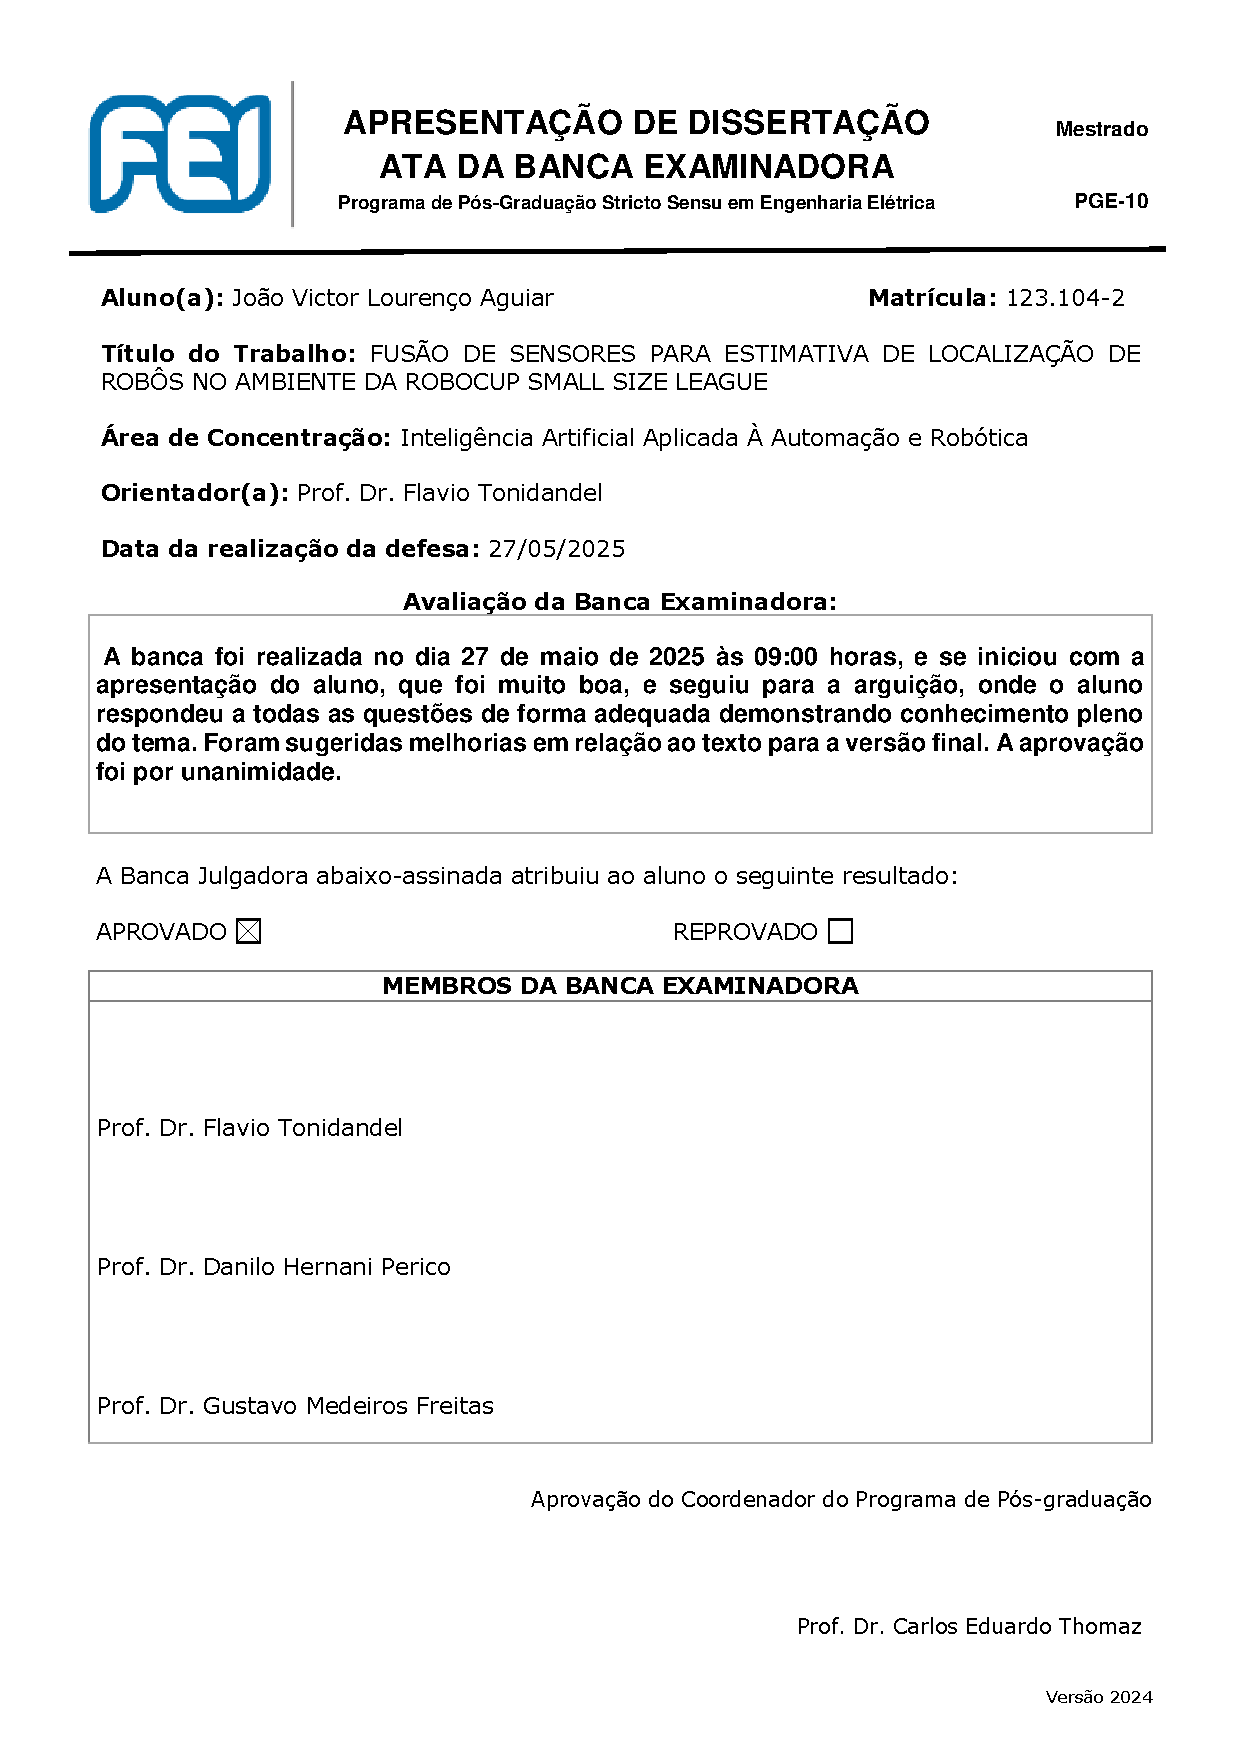
\includepdf{ata.pdf}\cleardoublepage
  \else
    \thispagestyle{empty}\mbox{}\vfill\begin{center}\begin{Huge}Folha de aprova\c{c}\~{a}o\end{Huge}\vfill\end{center}\cleardoublepage
  \fi
}

% ficha catalográfica: funciona da mesma forma da folha de aprovação, só que procura o arquivo *ficha.pdf*
\newcommand{\fichacatalografica}{
  \if@twoside
  \else
    % se não for frente e verso, a ficha catalográfica não é contada no verso da folha de rosto
    \addtocounter{page}{-1}
  \fi
  \ifdeposito
    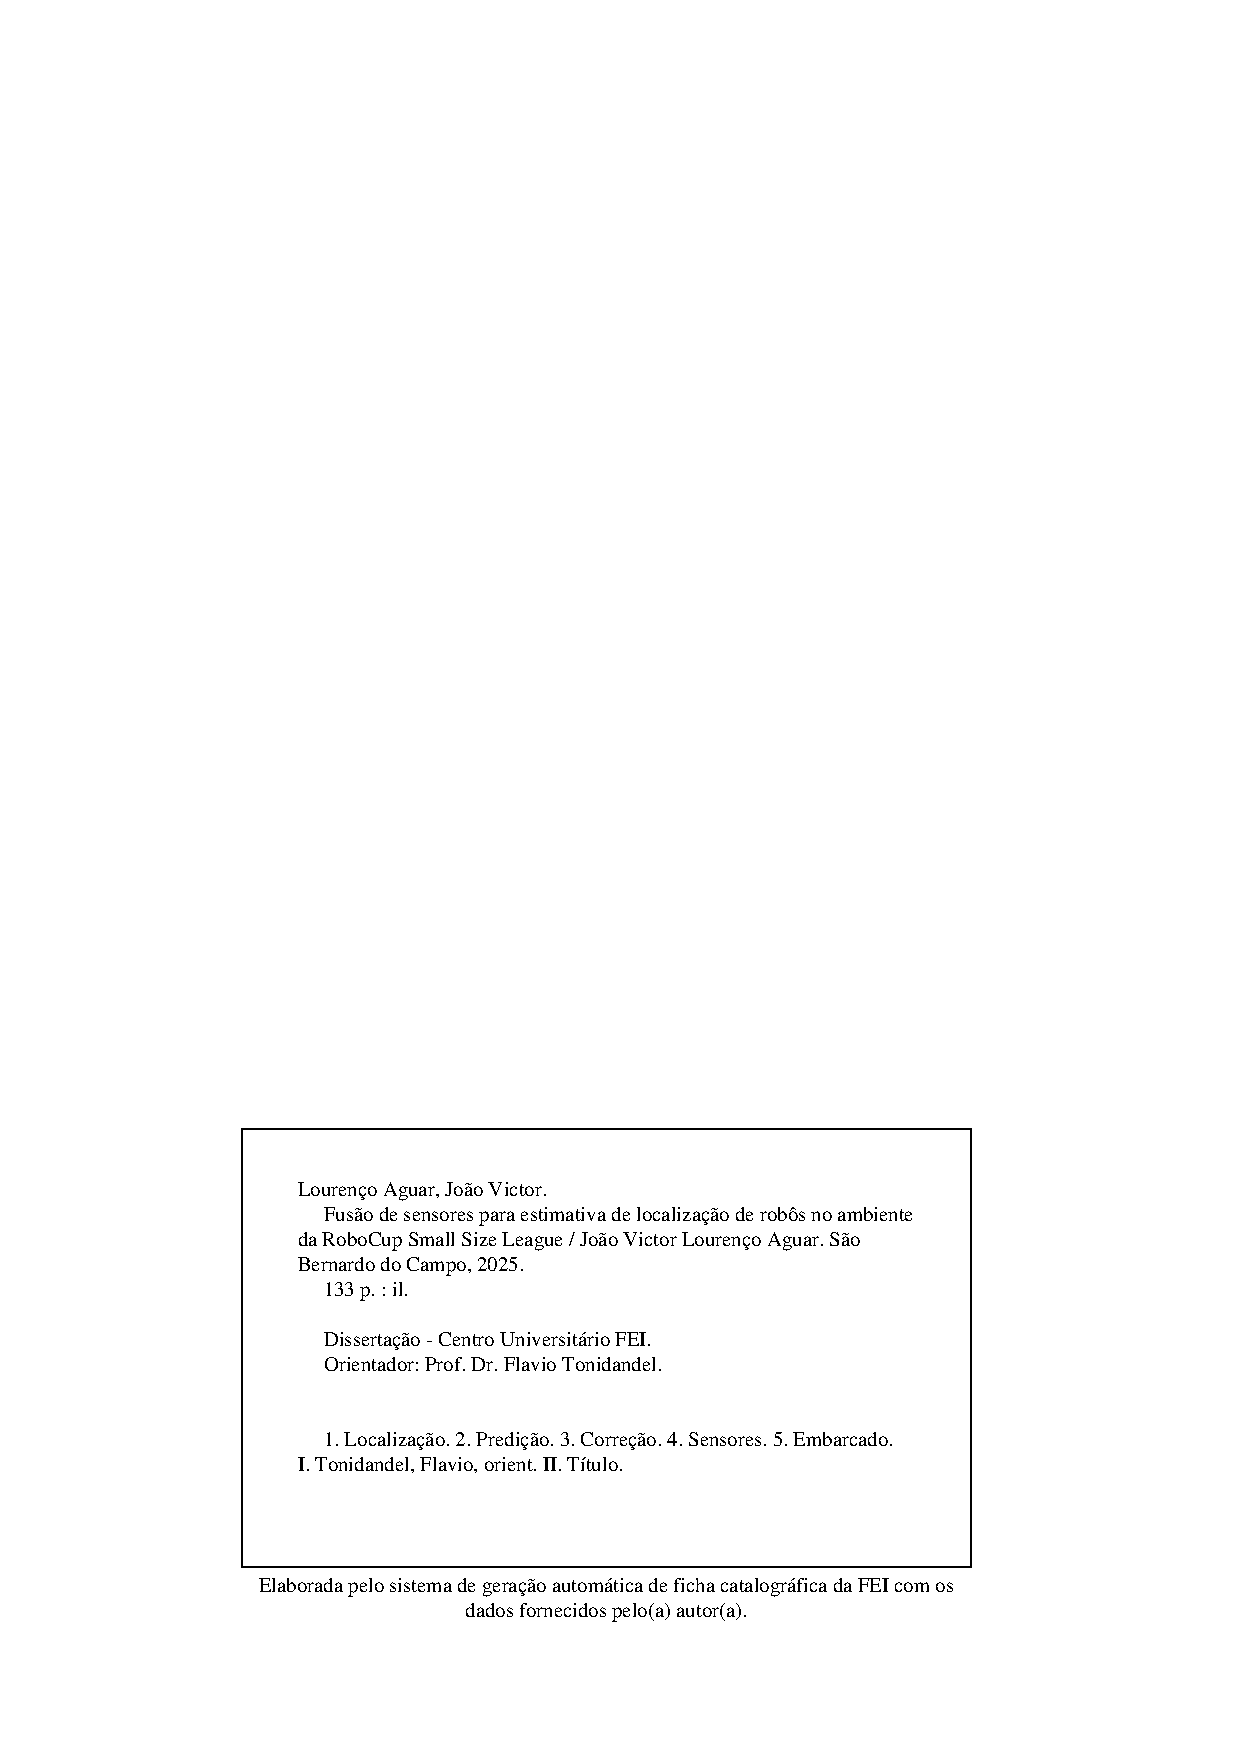
\includepdf{ficha.pdf}\cleardoublepage
  \else
    \thispagestyle{empty}\mbox{}\vfill\begin{center}\begin{Huge}Ficha catalogr\'{a}fica\end{Huge}\vfill\end{center}\cleardoublepage
  \fi
}

% subtítulo
\newcommand{\subtitulo}[1]{\def\@subtitulo{#1}}

\newcommand{\smallcaption}[1]{{\par\small%
      \begin{flushleft}#1\end{flushleft}}}

% cidade (padrão São Bernardo do Campo)
\def\@cidade{S\~ao Bernardo do Campo}
\newcommand{\cidade}[1]{\def\@cidade{#1}}

% instituicao (padrão Centro Universitário FEI)
\def\@instituicao{Centro Universit\'ario FEI}
\newcommand{\instituicao}[1]{\def\@instituicao{#1}}

% nome do orientador com respectivo título (ex Dr. ...)
\newcommand{\advisor}[1]{\def\@advisor{#1}}

% curso
\def\@curso{Coisa Nenhuma}
\newcommand{\curso}[1]{\def\@curso{#1}}

% dedicatória
\newcommand{\dedicatoria}[1]{
  \cleardoublepage
  \thispagestyle{empty}
  \vspace*{\fill}
  \begin{flushright}
    \begin{minipage}[t][0.5\textheight][c]{0.5\textwidth}
      #1
    \end{minipage}
  \end{flushright}
}

\newenvironment{epigrafe}{\cleardoublepage\thispagestyle{empty}\vspace*{\fill}}{}

\newcommand{\epig}[2]{
  \vspace{2\baselineskip}
  \begin{flushright}
    \begin{minipage}[t]{0.5\textwidth}
      ``{#1}''
      \begin{flushright}
        #2
      \end{flushright}
    \end{minipage}
  \end{flushright}
}
% resumo
\newenvironment{resumo}{\part*{Resumo}\pagestyle{empty}}{\cleardoublepage\setlength{\parindent}{1.25cm}}

% abstract
\renewenvironment{abstract}{\selectlanguage{english}\part*{Abstract}\pagestyle{empty}\setlength{\parindent}{1.25cm}}{\cleardoublepage\selectlanguage{brazil}}

% agradecimentos
\newenvironment{agradecimentos}{\part*{Agradecimentos}\pagestyle{empty}}{\cleardoublepage}

% índice
\RequirePackage[xindy]{imakeidx}
\indexsetup{level=\part*}
\addto\captionsbrazil{%
  \renewcommand{\indexname}{\'Indice}%
}

\let\oldprintindex\printindex
\renewcommand{\printindex}{\clearpage\phantomsection\addcontentsline{toc}{chapter}{\hspace{\cftchapternumwidth}\'INDICE}%
  \renewcommand{\chapter}{%
    \@startsection{chapter}{0}{0pt}{0pt}{1.5cm}{\clearpage\fontsize{12pt}{14.4pt}\bfseries\MakeUppercase}}%
  \oldprintindex%
}%

% antigamente, aqui era carregado o pacote hyperref.
% como, a partir de 2017, a biblioteca exige que os documentos sejam gerados sob o padrão
% PDF/A, o pacote pdfx é usado no lugar do hyperref por padrão
% em teoria, o pacote hyperref deveria ser o último a ser carregado, porém
% funcionou posicionado antes do glossaries, possibilitando links das variaveis para lista de simbolos
\ifpdfa
  \RequirePackage[a-1b]{pdfx}
\else
  \RequirePackage{hyperref}
\fi

% o pacote pdfx carrega o hyperref, então as opções do hyperref são passadas assim agora
\hypersetup{%
  pdftex,%
  pdfborder={0 0 0},%
  colorlinks={false},%
  % cria "bookmarks" no PDF até o 4° nível,
  % independente do valor de tocdepth, que eu mudo em alguns lugares
  bookmarksdepth=4%
}

% pacote para gerar listas (símbolos, abreviaturas, etc)
% glossaries-extra é usado pois permite incluir abreviaturas em seus idiomas originais
% para uma explicação melhor do motivo de se usar glossaries-extra, 
% este foi o problema que eu resolvi com ele: https://tex.stackexchange.com/a/77561/30998
\ifglossaries
  \ifsublist
    \RequirePackage[xindy,nomain,nonumberlist,section=part]{glossaries-extra}
    % estilo usado como base
    \setglossarystyle{alttree}
    % Configuracao de identacao do nivel 0 (titulos)
    \glssetwidest[0]{}
    % Configuracao de identacao do nivel 1 (a lista de simbolos em si)
    \glssetwidest[1]{aaaaaaaaaaaa}

    % remove número de página das listas de símbolos e abreviaturas (executado na primeira página)
    \renewcommand*{\glossarypreamble}{\thispagestyle{empty}\pagestyle{empty}\vspace*{-2\baselineskip}}

  \else
    \RequirePackage[xindy,nomain,nonumberlist,section=part,nogroupskip]{glossaries-extra}

    \newglossarystyle{mylong}{%
      \setglossarystyle{long}% base this style on the long style
      % \renewenvironment{theglossary}{%
      %   \begin{longtable*}{lp{\glsdescwidth}}}%
      %     {\end{longtable*}}%
    }%

    \setglossarystyle{long}
    \setlength\LTleft{0pt}
    \setlength\LTright{0pt}
    \setlength\glsdescwidth{\linewidth}

    % remove número de página das listas de símbolos e abreviaturas (executado na primeira página)
    \renewcommand*{\glossarypreamble}{\thispagestyle{empty}\pagestyle{empty}}
  \fi
  % traduz alguns comandos próprios do glossaries
  \addto\captionsbrazil{%
    \renewcommand*{\acronymname}{Lista de Abreviaturas}%
    \renewcommand*{\glssymbolsgroupname}{Lista de S\'imbolos}%
  }

  % redefine comandos do glossaries
  % remove número de página das listas de símbolos e abreviaturas (executado nas demais páginas)
  \renewcommand*{\glsclearpage}{\pagestyle{empty}}
  % remove número de página das listas de símbolos e abreviaturas (executado na última página)
  \renewcommand*{\glossarypostamble}{\pagestyle{empty}\cleardoublepage}
  % estilo das abreviaturas que permite imprimir a tradução de uma abreviatura em idioma estrangeiro
  \setabbreviationstyle[acronym]{long-short-user}
  % listas de simbolos e abreviaturas nao aparecem no sumario
  \glstocfalse

  % \glscurrentfieldvalue only works with glossaries v4.23 (and above)
  \renewcommand{\glsxtrpostdescacronym}{%
    \ifglshasfield{\glsxtruserfield}{\glscurrententrylabel}%
    { (\glscurrentfieldvalue)}%
    {}%
  }
\fi

\addto\captionsbrazil{%
  \renewcommand*{\listfigurename}{Lista de Ilustra\c{c}\~oes}%
  \renewcommand*{\contentsname}{Sum\'ario}}%

\newcommand{\palavraschave}[1]{\mbox{}\\\noindent Palavras-chave: #1}% o resumo pede palavras chave no final
\newcommand{\keywords}[1]{\mbox{}\\\noindent Keywords: #1}% mesma coisa, mas pro abstract

% referências e citações
% abnTeX alfabético com títulos das publicações em negrito nas referências (como no modelo antigo da ABNT)

\ifnumeric
  \RequirePackage[backend=biber,
    safeinputenc=true,
    uniquelist=false,
    doi=true,
    repeatfields=true,
    style=abnt-numeric]{biblatex}
\else
  \RequirePackage[backend=biber,
    safeinputenc=true,
    uniquelist=false,
    doi=true,
    repeatfields=true,
    style=abnt]{biblatex}
\fi

\setlength{\bibitemsep}{1.0\baselineskip}

\DefineBibliographyStrings{brazil}{%
  bibliography = {REFER\^ENCIAS}
}

% ###############################################################################
% Alterando o estilo biblatex-abnt
% 
% Encontrar os comandos nos seguintes arquivos e reescrevê-los aqui
% 
% Referências são impressas: https://github.com/abntex/biblatex-abnt/tree/master/latex/bbx
% Citações: https://github.com/abntex/biblatex-abnt/blob/master/latex/cbx/abnt.cbx
% Strings literais: https://github.com/abntex/biblatex-abnt/blob/master/latex/lbx/brazilian-abnt.lbx
% ###############################################################################

% remove <> das URLs (para a versão de 2019 da classe)
\DeclareFieldFormat{url}{\bibstring{urlfrom}\addcolon\addspace\url{#1}} %

\let\oldprintbibliography\printbibliography

\renewcommand{\printbibliography}{%
  \linespread{1}
  \oldprintbibliography
  \linespread{1.5}
}

\newcommand{\citeonline}[1]{\textcite{#1}}

% bibliografia alinhada à esquerda
% não é mais necessário na versão 3.1 do biblatex-abnt
% \renewcommand*{\bibfont}{\raggedright}

\defbibheading{bibliography}[\bibname]{%
  \clearpage\phantomsection\addcontentsline{toc}{chapter}{\bfseries\hspace{\cftchapternumwidth}REFER\^ENCIAS}% adiciona o titulo ao sumario
  \part*{REFER\^ENCIAS}
  \urlstyle{same}% URLs nas referências devem ter a mesma fonte do texto
}

% mantido para fins de compatibilidade com a versão 2 e 3 da classe
\newcommand*{\citefloat}[1]{\textcite*{#1}}

% modifica ambiente quote para citações de um parágrafo com mais de 3 linhas
\renewenvironment{quote}
{\begin{flushright}
    \begin{minipage}{\textwidth - 4cm}
      \fontsize{10pt}{1em}
      \begin{SingleSpace}
        }{\end{SingleSpace}\end{minipage}{}
  \end{flushright}}


% quotation é igual a quote, porém para citações com mais de um parágrafo.
\renewenvironment{quotation}
{\begin{center}
    \begin{minipage}{\textwidth - 4cm}
      \fontsize{10pt}{1em}
      \begin{SingleSpace}\setlength{\parindent}{1cm}
        }{\end{SingleSpace}\end{minipage}{}
  \end{center}}
%</class>
